\chapter{Language games}\label{ch:lg}\label{ch:cm}
\section{Introduction}

In order to solve the symbol grounding problem the robots engage in a series of language games. Every language game can be thought of as a communication act in which the robots communicate about an object (in this case a light source). The goal of a language game is for the two robots to identify the same referent through the exchange of linguistic and possibly non-linguistic information. If this does not succeed they can adjust their set of meanings and/or lexicons so they may be successful in future games.


\index{Wittgenstein, Ludwig|(}
The notion of a language game was first introduced by Ludwig \citet{wittgenstein:1958}. Wittgenstein called every language use a language game. The meaning of the language game depends, according to Wittgenstein, on the {\em how} the game is used. Wittgenstein gave some examples of different types of language games \cite[11, §22]{wittgenstein:1958}:

\begin{quote}
\begin{itemize}
\item Giving orders, and obeying them
\item Describing the appearances of an object, or giving its measurements
\item Constructing an object from a description (a drawing)
\item Reporting an event
\item Speculating about an event
\item \ldots 
\end{itemize}
\end{quote}

In the experiments done at the \textsc{ai} Lab different types of games are investigated. Besides the basic term of language game, the following games have been introduced {\scshape naming games} \citep{steels:1996a}, {\scshape discrimination games} \citep{steels:1996b}, {\scshape imitation games} \citep{deboer:1997}, {\scshape guessing games} \citep{steelskaplan:1999}, {\scshape identification games} and {\scshape follow me games} \citep{vogt:1999a,vogt:2000}. All games model a communication act, except the discrimination and identification games which model categorisation. The types of games that will be used in this book are naming games, discrimination games, guessing games and two additional games that will be explained further on in this chapter. The discrimination and naming game form a sub-part of what is called a language game here. The other games are a special type of language game.

\index{Wittgenstein, Ludwig|)}


In the context of this work, a language game is the complete process of performing a communication act. As mentioned in \chapref{ch:intro}, grounding language is strongly influenced by an agent's interaction with its environment. Since it is assumed that language and meaning formation are complex dynamical adaptive systems, these systems can be defined by their mechanical processes and the systems boundary conditions \citep{prigogine}. So, to develop a robot capable of constructing conceptual structures and language, one has to define such mechanisms and boundary conditions of the system. The mechanism has already been chosen, namely the {\scshape selectionist approach} taken \citep{steels:1996a,steels:1996b}. The boundary conditions will be defined (for a great deal) by the {\scshape physical bodies} and {\scshape interaction} of the robots with their ecological niche. 


This chapter presents the physical interactions of the robots with their environment. It defines the language game scenario in detail, defining the physical interaction in which a context setting is acquired. This happens in the next section. Then \sectref{s:lg:offboard}\todo{unknown target for sectref} discusses the advantages of on-board vs. off-board processing as a methodology of experimenting with robots.  \sectref{s:lg:perception} discusses the perception and segmentation during a language game. Sections \ref{s:cm:dg} and \ref{s:cm:ng} explain the higher cognitive functions of categorisation and naming. A final section of this chapter couples the different parts of the language game.


\section{The language game scenario}\label{s:lg:scenario}

\index{language!game|(}


The goal of a language game is to communicate a name for one of the light sources that the robots can detect in their environment. To do so, both robots first have to sense their surroundings. One of the robots takes the role of the speaker, the other takes the role of hearer. The speaker selects one sensation of a light source. This light source is the subject of the communication. The speaker looks for a category that relates to the sensation of this light source. When it did this, it searches a word-form that it has associated with this category in the past. This word-form is then communicated to the hearer. 

The hearer, who has also sensed several light sources, tries to interpret the communicated word-form. It looks in its memory if it had stored an association of this word-form with one or more meanings that relate to the sensation of the light sources. If the hearer can find a link between the word-form and some light source, the language game is successful when both robots communicated about the same light source.

In the beginning of the experiments, the robots have no categories or word-forms yet. These are the things that they need to develop. So, when the robots are not able to find a suitable category or a word-form, they may expand their memory in order to do so in the future. And if they were able to do so, they will increase the strength of the used association, which increases the chance that they will be successful in the future. How they do this will be explained in detail in this chapter. In this section, the sub-tasks of a language game will be identified and organised.

\begin{table}
\centering
\begin{tabular}{cc}
\lsptoprule
{\sc speaker} & {\sc hearer}\\
\midrule
\multicolumn{2}{c}{{Get together and align}}\\\hline
\multicolumn{2}{c}{Sensing, segmentation and feature extraction}\\\hline
Topic choice & --\\\hline
{Pointing} & {Topic selection}\\\hline
\multicolumn{2}{c}{Categorisation}\\\hline
Production & --\\\hline
-- & Understanding\\\hline
\multicolumn{2}{c}{Feedback}\\\hline
\multicolumn{2}{c}{Adaptation}\\\lspbottomrule
\end{tabular}
\caption{The language game scenario. The ``Get together and align'' phase is done by the experimenter for practical reasons. ``Pointing'' and ``Topic selection'' may be omitted for methodological reasons. See the text for more details.}
\label{t:scenario1}
\end{table}


So, how is a language game organised? \tabref{t:scenario1} shows the structure of the language game scenario. In a language game two robots -- a {\scshape speaker} and a {\scshape hearer} -- get together at close distance. In earlier experiments \citep{steelsvogt:1997} the robots came together autonomously. When sensing each other's vicinity, the speaker approached the hearer by using infrared phototaxis. When both robots were close to each other, they aligned such that they faced each other prior to the sensing. This behaviour, however, took approximately 1.5 minutes for each language game. To speed up the current experiments the robots have been brought together manually. The {\sc pdl} source code for finding each other is included in Appendix \ref{a:pdl}. For more details on this part of the language games, consult \citealt{vogt:1997}.  

When the robots are standing together at close distance, they acquire a spatial view of their surroundings by means of a specialised sensing task. This sensing task results in a spatial view of the robot's surroundings, which is then segmented resulting in a {\scshape set of segments} (or {\scshape context} for short). Each segment is supposed to refer to a light source as detected by the robot and is represented by a set of connected data points. These data points are sensory data that from which the noise is reduced. From these segments feature vectors are extracted that designate some properties of these segments. 

The speaker chooses one segment from the context to be the topic of the language game and tries to categorise its relating feature vector by playing a discrimination game. The discrimination game results in one or more distinctive categories. The hearer identifies one or more segments from the context as a possible topic an tries to categorise its (their) related feature vector(s).

After the speaker has chosen a topic and categorised this segment, it produces an {\scshape utterance}. An utterance is the communication of a form. The hearer tries to understand this utterance by looking for matching associations of this form with a meaning in its lexicon. If one of these meanings is coherent with one of the distinctive categories of the topic, then the language game {\it may} be a success. The language game is {\scshape successful} when the speaker and the hearer communicated about the same referent. The evaluation of the success is called the {\scshape feedback}.

If the language game was not a success, the lexicon has to be adapted either by creating a new form (if the speaker could not produce an utterance), by adopting the form (if the hearer could not understand the utterance) or by decreasing association scores. Association scores are increased when the language game is successful. The process that models naming and {\scshape lexicon adaptation} is called a naming game. \figref{f:scheme} illustrates the language game scenario schematically.

\begin{figure}
\centering
\subfigure[]{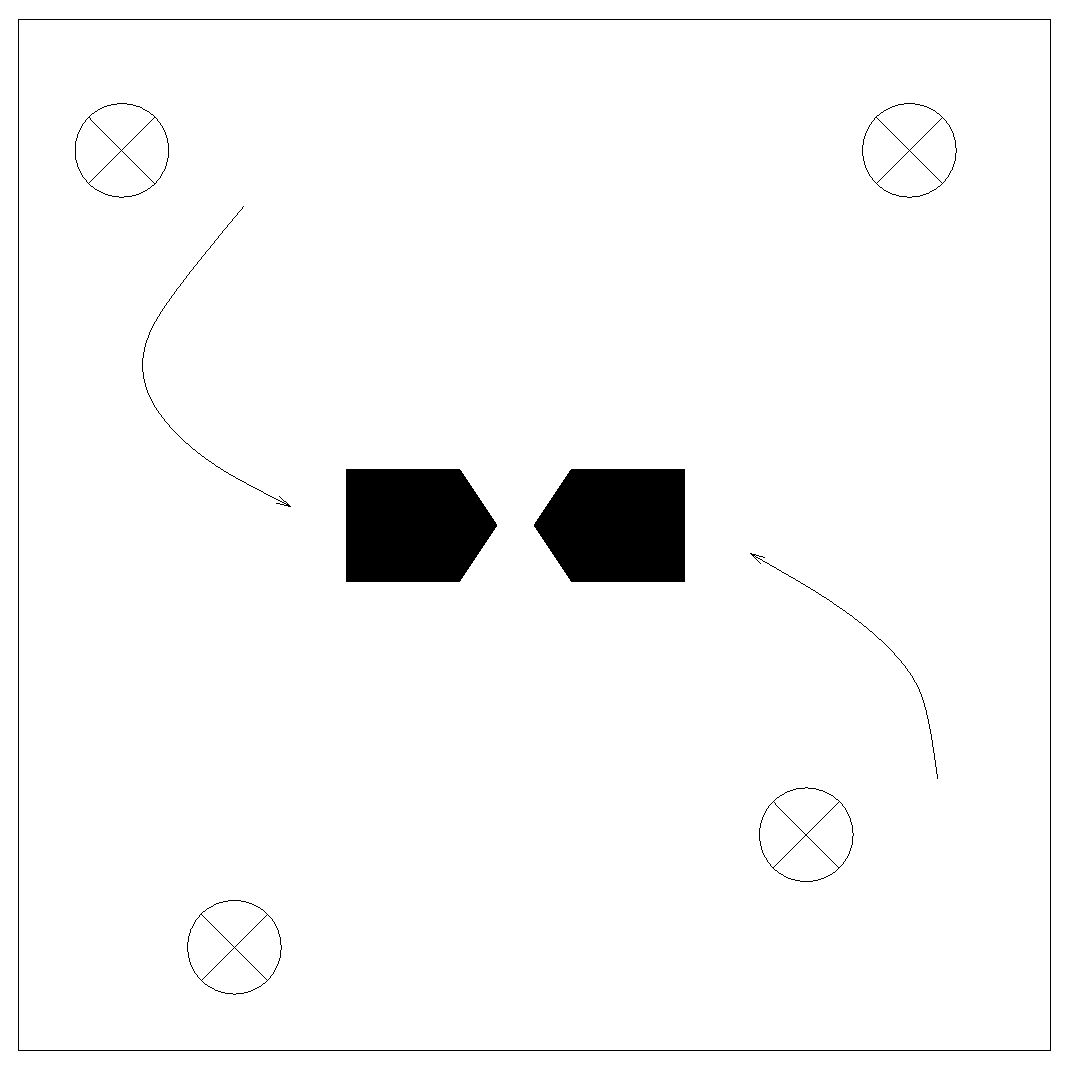
\includegraphics[width=5.5cm]{lang_games/schema0.eps}}
\subfigure[]{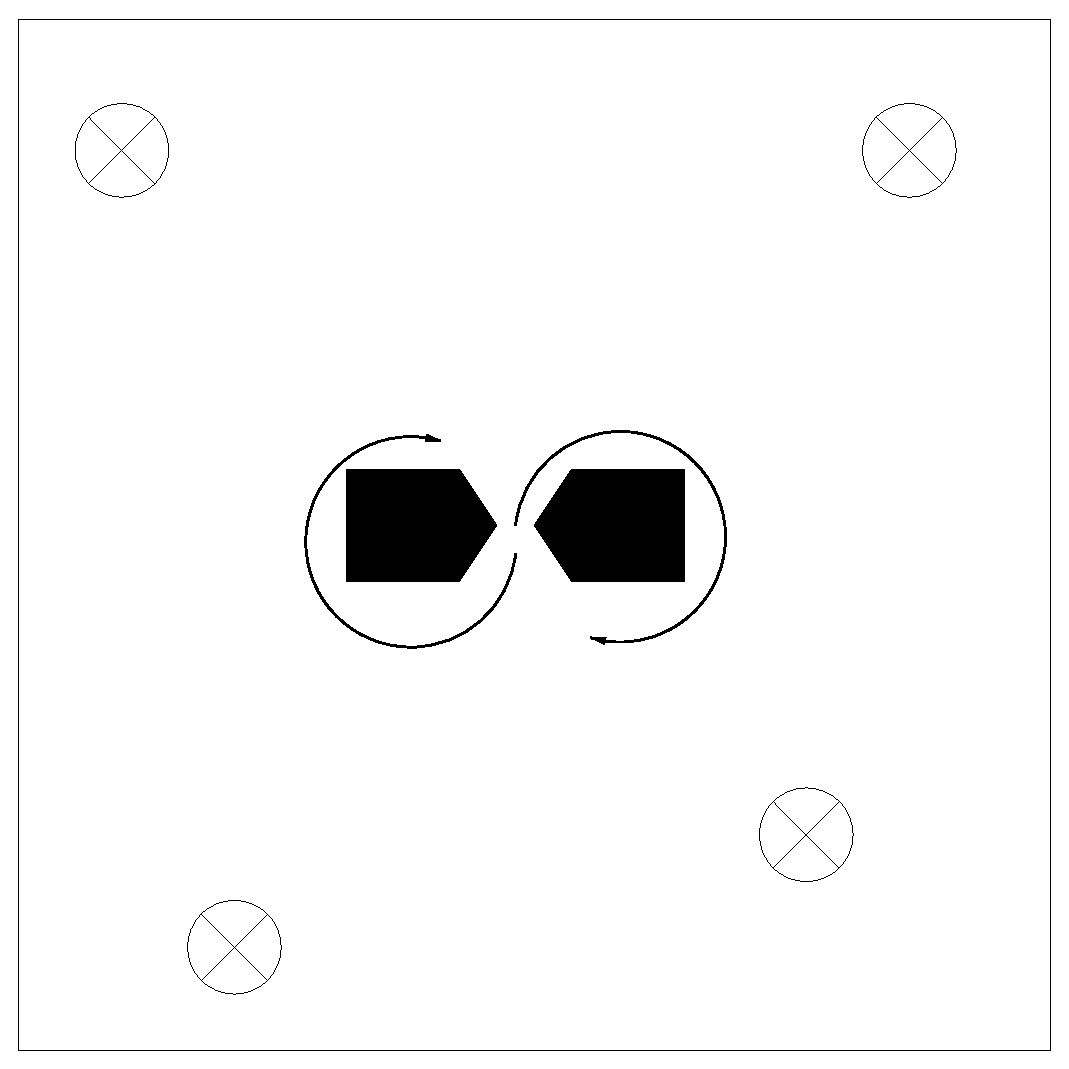
\includegraphics[width=5.5cm]{lang_games/schema1.eps}}\\
\subfigure[]{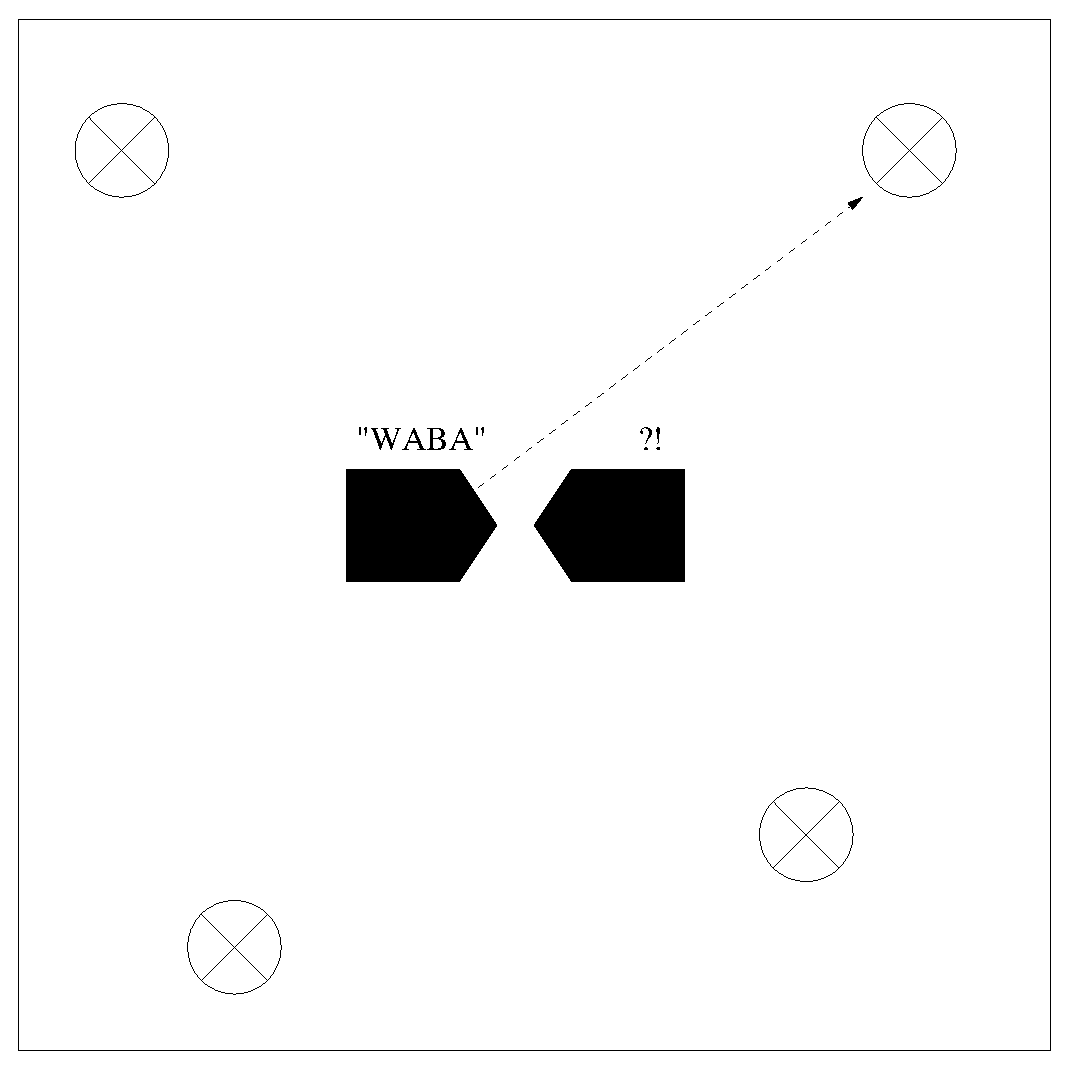
\includegraphics[width=5.5cm]{lang_games/schema2.eps}}
\subfigure[]{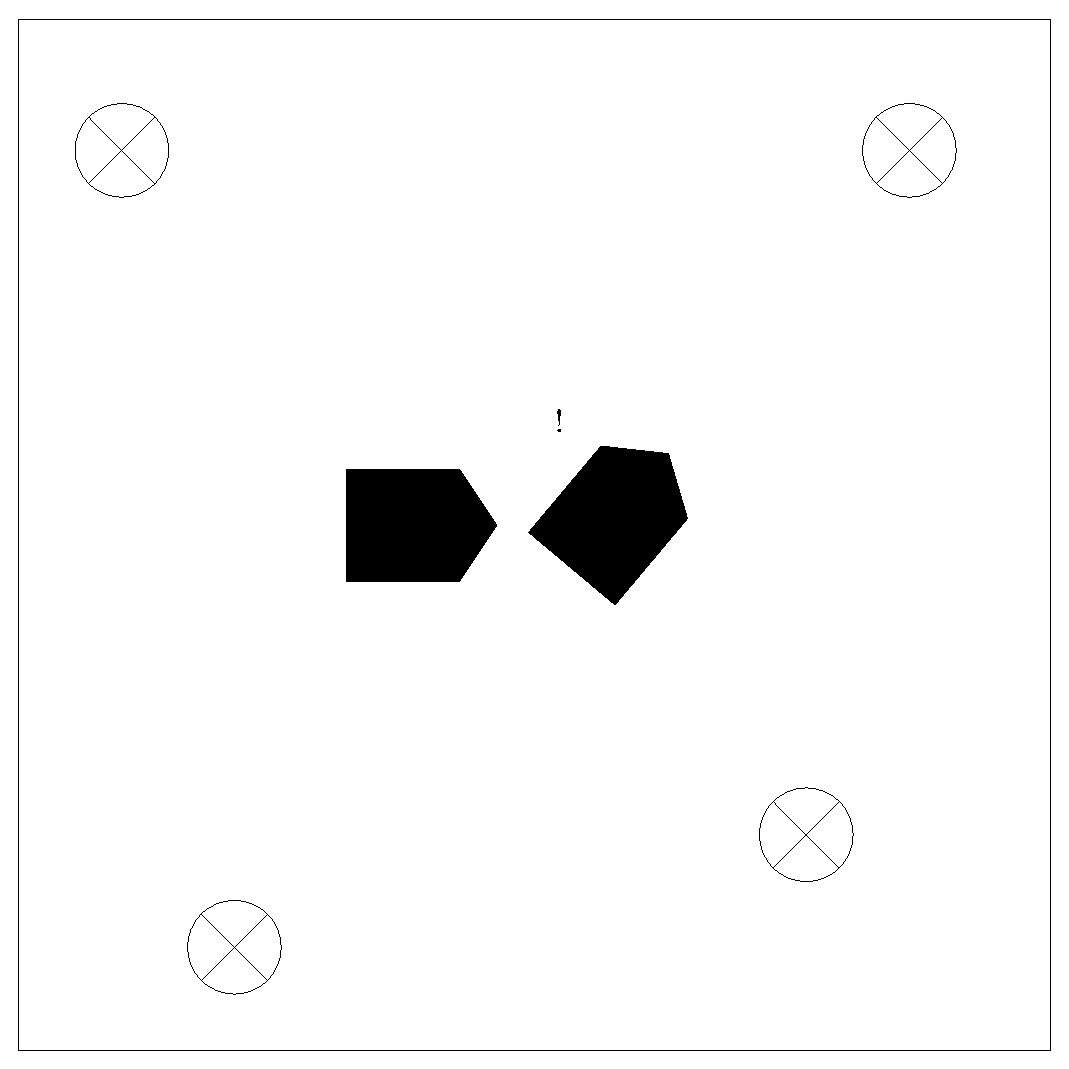
\includegraphics[width=5.5cm]{lang_games/schema3.eps}}
\caption{A temporal overview of the language game scenario. (a) The robots get together aligned and align. (b) The robots rotate in order to sense their surroundings. (c) The speaker produces an utterance and the hearer tries to understand the speaker. (d) When the hearer ``thinks'' it understood the speaker, feedback is established and the robots' memories are adapted.}
\label{f:scheme}
\end{figure}

\section{PDL implementation}

\index{PDL|(}\index{behaviour-based!cognitive architecture|(}
To play a language game, a robot has to perform a sequence of actions. These actions need to be planned. The planning is pre-programmed as a script using finite state automata. There is a finite state automaton ({\sc fsa}) for each role the robots can play: the speaker or hearer. Each finite state automaton is active all the time and when no language game is played, both robots are in state 0. A process called \texttt{DefaultBehavior} decides when an agent goes into state 1 of the speaker-{\sc fsa} or hearer-{\sc fsa}. In each state a set of dynamic processes is activated or inhibited.\footnote{See \chapref{ch:robots} for a general presentation of the behaviour-based cognitive architecture.}

How the physical behaviours of the robots are implemented in {\sc pdl} is presented in Appendix \ref{a:pdl}. \sectref{s:lg:grounded} sketches the architecture as a general architecture for developing cognitive robots. After the introduction of the architecture sensing, segmentation and pointing is discussed in detail.

\begin{figure}
\centerline{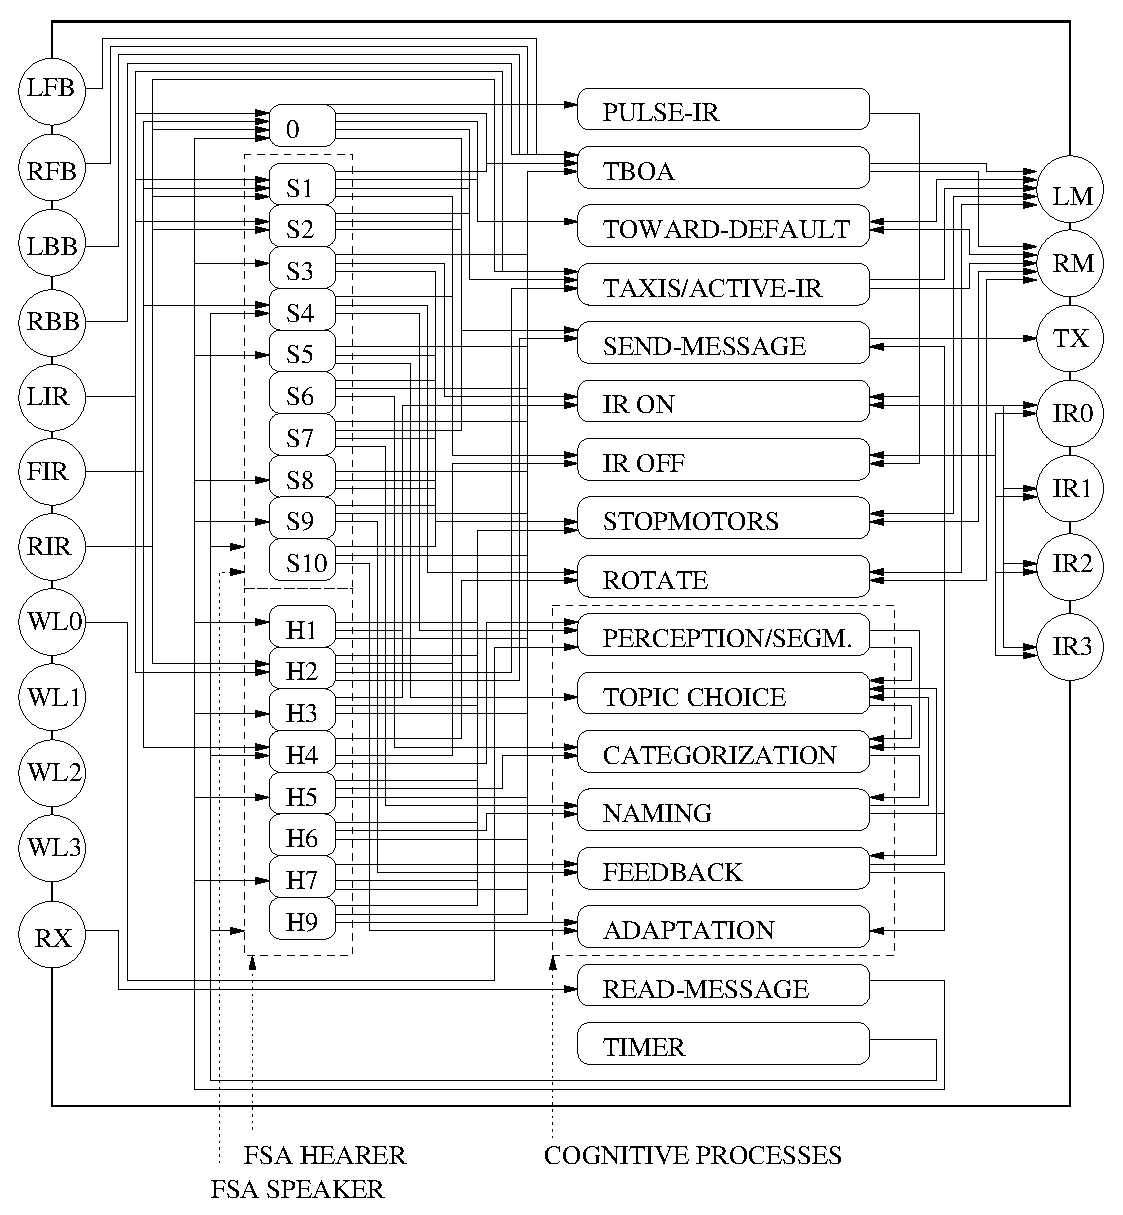
\includegraphics[width=12cm]{lang_games/architecture.eps}}
\caption{The behaviour-based cognitive architecture of the robotic system for processing language games. Note that the {\sc pdl}-like network structure as introduced in \sectref{s:robots:pdl}. The flow of information follows each line in the direction of the arrow. If a cross-connection is found, the information follows the line straight. Only when a T-connection is encountered, the direction of the arrow is taken. Some lines are bi-directional, in such cases information flows in both directions. Basically, the information flows from the sensors on the left-hand side of the figure to the actuators on the right-hand side. In between, the information first flows in the finite state automata that controls the planning of the robots. \tabref{t:abbr} gives the translation of the abbreviations. Note that the term ``perception'' is used to designate the sensing.}
\label{f:architecture}
\end{figure}

\begin{table}
\centering
\begin{tabular}{>{\scshape}ll}
\lsptoprule
\multicolumn{2}{c}{{\sc sensors}}\\
\midrule
lfb & Left Front Bumper\\
rfb & Right Front Bumper\\
lbb & Left Back Bumper\\
rbb & Right Back Bumper\\
lir & Left Infrared Sensor\\
fir & Front Infrared Sensor\\
rir & Right Infrared Sensor\\
wl & White Light Sensor\\
rx & Radio Receiver\\
\midrule
\multicolumn{2}{c}{{\sc finite state automata}}\\
\midrule
0 & Default State\\
{\rmfamily Sx} & Speaker's State x\\
{\rmfamily Hx} & Hearer's State x\\
\midrule
\multicolumn{2}{c}{{\sc processes}}\\
\midrule
tboa & Touch-Based Obstacle Avoidance\\
\midrule
\multicolumn{2}{c}{{\sc actuators}}\\
\midrule
tx & Radio Transmitter\\
lm & Left Motor\\
rm & Right Motor\\
ir & Infrared Emitter\\
\lspbottomrule
\end{tabular}
\caption{\todo[inline]{move this to abbreviations.tex?}A list of abbreviations as used in \figref{f:architecture}.}
\label{t:abbr}
\end{table}


\figref{f:architecture} shows how the language games are implemented in the behaviour-based cognitive architecture. The architecture is built of a large set of parallel processes, which are continuously being processed. These processes, however, do model different types of behaviour and should not be viewed at one level of complexity. Rather, the processes are organised hierarchically. 

There is a finite state automaton for the speaker role and one for the hearer. Each state of the finite state automaton activates a set of processes that are shown to the right of the finite state automaton. Those processes that are active respond to information that flows from connected sensors, actuators or other processes. All processes have been implemented in {\scshape pdl} on the real robots in previous versions \citep{steelsvogt:1997}. In the current experiments, the cognitive processes are implemented as software agents that are processed on a {\scshape pc}.

There are reactive processes like taxis, rotate and obstacle-avoidance. All these processes guide the physical behaviour of the robots.

The cognitive processes can be distinguished from the reactive processes in that they model more complex behaviour and need not directly influence actuators, but they can also influence the internal state of an agent.\footnote{Although the term ``cognitive processes'' is sometimes used to refer to reactive processes as well, the term is used here to indicate the distinction between reactive behaviours and behaviours that require more sophisticated cognitive processing. The cognitive processes refer to those processes that are fundamentally involved in categorisation and/or naming.} Coincidentally all cognitive processes are implemented off-board, besides the sensing which is implemented on-board. The cognitive processes tend to work at different time scales then reactive ones. I.e. the time necessary to, e.g., categorise something takes computationally longer than reactive responses do. This has not only been observed in neuroscience,\footnote{There is a lot of evidence for fast and slow pathways in the central nervous system, where the fast pathways are reactive and the slow are considered to model higher cognition (see e.g. \citealt{ledoux:1996}).} but also during the implementation of so-called follow me games \citep{vogt:1999a,vogt:2000}\index{follow me game}. In the follow me games the hearer is following the speaker using phototaxis. When a change in direction is encountered the robot categorises a part of its movement. If both phototaxis and categorisation and naming are processed simultaneously on the {\sc smbii}, the robot fails to follow the speaker because the categorisation process takes more time than $0.025 s$, which is the time of one {\sc pdl} cycle. Although {\sc pdl} normally cycles the read-process-execute cycle 40 times per second, it only does so when it finished all its processes. 

The categorisation and naming are single processes that carry out a complex process of search, selection and adaptation, but these processes could in principle be modelled by a set of parallel processes as well. This has not been done for the sake of both simplicity and architectural requirements (the computers used are still serial machines).

Both the reactive and cognitive processes are activated or inhibited by the motivational factors which are set inside the states of the finite state automaton. So, depending on the role an agent has, it will enter either the speaker-{\sc fsa} or the hearer-{\sc fsa}. Each finite state automaton models a script-like scheme that takes care of the plan. Note that of course, depending on the task, numerous finite state automata could be developed. Each state takes either direct sensory stimuli or indirect stimuli as read messages or a timer as their arguments. These stimuli are used to determine when the final condition of the state is reached. The final conditions of a state are immediately the initial conditions of the next state. If a robot is too long in one state, measured by the timer, a transition is made to the default state and consequently the language game fails. All other final conditions cause the robot to enter the subsequent state unless it is the final state of the automaton, then it also enters the default state. If no final condition is met, the robot remains in (or re-enters) the same state.

This section\todo{this chapter?} sketched how language games are implemented in the behaviour-based cognitive architecture. Of course, much more could be said about the architectural implementation, but this is beyond the scope of the dissertation, which is more concerned with grounding symbols.
\index{PDL|)}\index{behaviour-based!cognitive architecture|)}

\section{Grounded language games}\label{s:lg:grounded}

How are the different sub-parts of the language game scenario modelled? Up to now the physical set-up and implementation of the robots and their interactions have been explained. The only part of the implementation that still needs to be presented are the cognitive models that implement the sensing, segmentation, feature extraction, categorisation and lexicon formation. These models are the core of the present solution to the physical symbol grounding problem. The remainder of this chapter presents these processes.

Sensing, segmentation and feature extraction are important ingredients of the solution of the symbol grounding problem: they form the first step towards invariance. Invariance returns in the cognitive processes during the selection of elements. The three recognised problems in the symbol grounding problem iconisation, discrimination and identification \citep{harnad:1990} are cognitively modelled. Recall from \chapref{ch:intro} that iconisation is the construction of iconic representations that relate to the detection of some real world object. In these experiments, iconisation is more or less modelled by the sensing and segmentation. \citet{harnad:1990} calls ``discrimination'' the process where it is determined how iconic representations differ. He uses discrimination at the sensing level. Here discrimination is used at the categorisation level. It is modelled by the discrimination games. Identification is the process where categories are identified that relate to the iconic representations invariantly. This is modelled in this book by the naming game model. As will be explained soon, this classification is not so clear-cut.

As argued in \chapref{ch:intro}, a symbol can be illustrated with a semiotic triangle. The semiotic triangle, a symbol or sign has three relations: (1) meaning -- referent, (2) form -- meaning, and (3) form -- referent. So, how do robots that have no knowledge construct a meaningful ontology and lexicon for these three relations? Two models have been proposed to solve this problem. For relation (1), there are discrimination games \citep{steels:1996b}. Relation (2) is modelled by the naming game \citep{steels:1996a}. Coupling the two models in a grounded experiment provides relation (3). As argued in \chapref{ch:intro}, this is because language and meaning co-evolve \citep{steels:1997a}. Closing the semiotic triangle with success is then what \citet{harnad:1990} called ``identification'' and the symbol grounding problem is solved for that particular symbol. This is so, because only if it is closed successfully, there is enough reason to assume that the symbol stands for the referent.\index{symbol grounding problem!identification}

In the semiotic triangle there is a direct relation between meaning and the referent. However, in cognitive systems there is no such direct relation; the world has to be sensed first. So, to achieve a semiotic coupling, \citet{steels:2000} proposes a semiotic square rather than a triangle (see \figref{f:cm:semiotic}). Note that the square couples the semiotic relations in one robot with another. As argued, language dynamics is thought to give rise to the development of both the lexicon as the ontology. How the ontology and lexicon are developed is explained in Sections~\ref{s:cm:dg} and~\ref{s:cm:ng}. \sectref{s:lg:perception} explains how the robots do their sensing, segmentation and feature extraction.

\index{semiotic landscape}

\begin{figure}[t]
\centerline{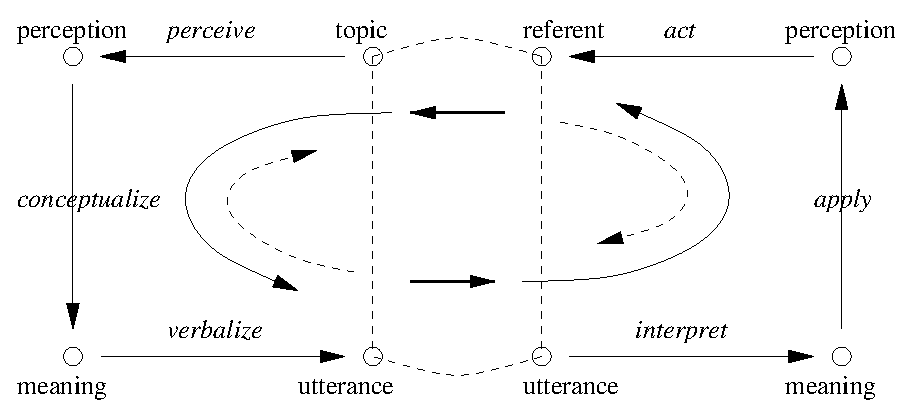
\includegraphics[width=12cm]{discr_games/semiotic1.eps}}
\caption{The semiotic landscape of a language game can be viewed as a structural coupling. In this landscape, there are two squares, representing the speaker (left) and the hearer (right). The speaker senses a topic, resulting in a perception. In the terminology of this book, this is called sensing. The perception is conceptualised (or categorised) yielding a meaning. This meaning is then verbalised by the speaker and when the hearer receives the utterance (or form), it tries to interpret this. The interpretation results in a meaning which can be applied to a perception. According to this perception, the hearer acts to identify the referent, which should be the same as the topic and thus completing the coupling. When at some point something goes wrong, the agent can adapt their memory. The errors are signalled by means of back propagation. The figure is taken from Steels 1999.\todo[inline]{there is no Steels 1999 in Bib}\index{semiotic landscape}}
\label{f:cm:semiotic}
\end{figure}

\subsection{Sensing, segmentation and feature extraction}\label{s:lg:perception}


In the phase of sensing, the goal is that each robot observes its surroundings from its current physical position. To obtain a more or less identical view, the robots start close to each other. Sensing its surroundings means that the robots construct a spatial view of their environment. This spatial view is represented by the recorded sensory data. However the robots cannot obtain a spatial view directly with the sensors they have, because the sensors can only detect light intensity without spatial information. In order to get a spatial view of their environment, either the robots need to have a spatially distributed array of sensors or the robots need to move. Because of the robots' physical limitations (and the sensory-motor board in particular) it is opted to let the robots move. As a side-effect a higher resolution is obtained. To obtain a spatial view of their complete surroundings the robots rotate a full circle around their axis.

The robot's observation of its surroundings results in a set of raw sensory data that represents the scene. However, in order to identify the different light sources, the robots have to find connected regions of the sensory data that relate to the sensing of these light sources. This is done by the {\itshape segmentation} process. The segmentation can result in segments of varying length. To be able to identify a good category it is more efficient to have a description in a consistent manner that designates invariant and useful properties or features of the sensation of the light source. Extracting these features is done by means of what is called {\scshape feature extraction}.

The detection of the raw sensory data is done completely on-board. This data is sent to a {\scshape pc} where it is processed further. So, the segmentation and feature extraction takes place on a {\scshape pc}. This is not necessary but convenient for reasons mentioned above.

\subsubsection{Sensing}
\index{sensing|(}

During the sensing, the robots construct a spatial view of their surroundings. But because the sensors cannot detect spatial information, sensing is done by letting the robots rotate (ideally) $360^o$ and record their sensory information while doing so. While they rotate (one by one) they record the sensor data 40 times per second. Each sensor writes its data on a {\scshape sensory channel}. The data that enter the sensory channels is transmitted to the {\scshape pc} via the radio.

\begin{figure}
\centerline{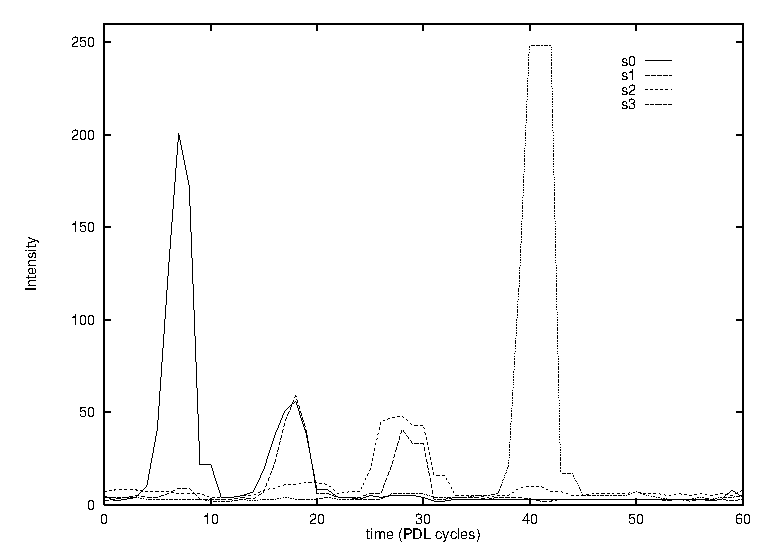
\includegraphics[width=9cm]{lang_games/perception1.eps}}
\caption{The sensing of a robot's surroundings as in the experiments. See the text for explanation.}
\label{f:perception1}
\end{figure}

\index{correspondence|(}

\figref{f:perception1} shows a spatial view of a robot's sensing. The sensing took 60 {\sc pdl} cycles ($=1.5 s$). Each peak {\em corresponds} to one of the four light sources in the environment. Remember that corresponding means that the sensor with the highest intensity at a peak detects the light source that is placed at the same height as the sensor itself. Recall that the environment consists of 4 light sources that are placed at different heights (\sectref{s:robots:robots}). 

\figref{f:perception1} shows that at time step $7$ sensory channel $s0$ sensed a large peak, whereas the other sensory channels show low peak values. At time step $18$ there is a main peak  for sensory channel $s1$ with lower peaks for the other sensory channels. Sensory channel $s2$ shows a maximum at time $28$ and sensory channel $s3$ sensed a maximum during time steps $40$ to $43$. Table \ref{t:perception1} gives these peaks with their sensory channel values.

\begin{table}
\centering
\begin{tabular}{crrrrr}
\lsptoprule
P & $t$ & $s0$ & $s1$ & $s2$ & $s3$\\
\midrule
1 & 7 & 201 & 9 & 7 & 3\\
2 & 18 & 56 & 59 & 11 & 3\\
3 & 28 & 5 & 41 & 48 & 6\\
4 & 42 & 3 & 3 & 10 & 248\\
\lspbottomrule
\end{tabular}
\caption{Peaks P observed in \figref{f:perception1}. The table lists the highest intensity reached at time $t$ with sensory channels $s0$, $s1$, $s2$ and $s3$.}
\label{t:perception1}
\end{table}

These peaks can all be explained with the characteristics of the sensory channels seen in \figref{f:robots:calibration}, page \pageref{f:robots:calibration}.  The intensity of each peak is dependent on the distance of the robot to the light source. The robot clearly detects light sources $L0$ and $L3$ from nearby; the corresponding sensory channels detect high values and almost all other sensory channels show low noise values. Light sources $L1$ and $L2$ are further away. The corresponding light sensors show relative low values and some adjacent sensory channels show values that are close to the corresponding sensory channels. Values lower than $10$ between the peaks are noise values.
\index{region of interest}
\index{correspondence|)}

\begin{figure}
\centerline{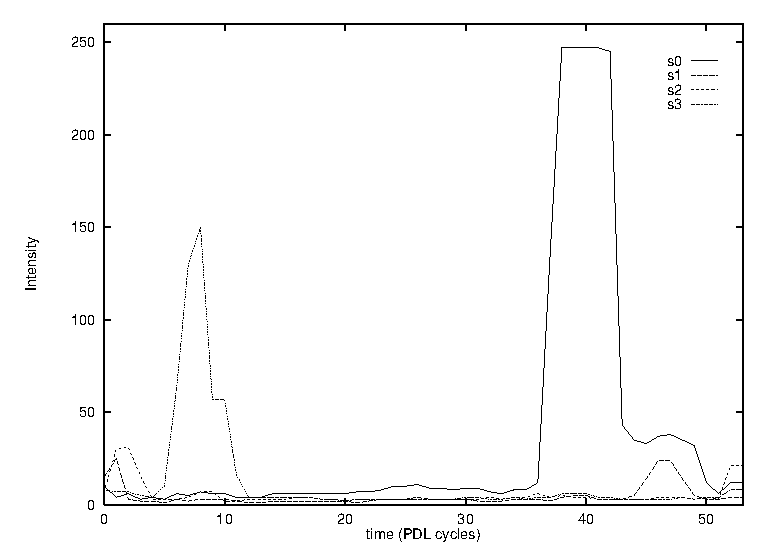
\includegraphics[width=9cm]{lang_games/perception2.eps}}
\caption{The sensing of the hearer in the same language game situation as in \figref{f:perception1}.}
\label{f:perception2}
\end{figure}


After the speaker finished its sensing, the hearer starts its sensing. That the hearer does not sense the same view as the speaker can clearly be seen in \figref{f:perception2}, which shows the spatial view of the hearer during the same language game. If one looks carefully, one can see similarities, but there is no straightforward mapping. In this plot five interesting peaks can be identified (see \tabref{t:perception2}).

\begin{table}
\centering
\begin{tabular}{crrrrr}
\lsptoprule
P & t & $s0$ & $s1$ & $s2$ & $s3$\\
\midrule
1 & 1 & 4 & 25 & 30 & 7\\
2 & 8 & 7 & 3 & 7 & 150\\
3 & 40 & 247 & 5 & 4 & 6\\
4 & 47 & 38 & 24 & 4 & 3\\
5 & 54 & 12 & 4 & 21 & 8\\
\lspbottomrule
\end{tabular}
\caption{Peaks of \figref{f:perception2}.}
\label{t:perception2}
\end{table}

Peaks 1 and 5 (\tabref{t:perception2}) both appear to correspond to $L2$. Although the times at which the peaks are observed lie far apart, these peaks are detected under almost the same orientation of the robot, namely in the front. This fits well with the sensing of $L2$ of the speaker as shown in \figref{f:perception1}, where it is behind the speaker. Peaks 2 and 3 (corresponding to $L3$ and $L0$ resp.) can also be well related to the sensing of the speaker. 

Peak 4, which is just observable after the largest peak (between time 55 and 60), does not clearly correspond to a light source. One would expect to detect $L1$, both intuitively as from the sensing of the speaker. Sensory channel $s1$ does indeed show a peak here, but $s0$ shows the highest peak. Peak 4 is also interesting from another point of view. As will be shown below, the segmentation will not recognise this segment. According to the definition just given, it is part of the same region of interest as peak 3 because the intensity does not drop below the noise value.


Usually, the sensing takes about 1.5 seconds, so the robots obtain approximately 60 subsequent data points. Since the robots have 4 sensory channels, they will have a spatial view of about $60 \cdot 4$ data points. Because the speed of rotation is not always constant and it also varies depending on the energy level of their batteries, the number of data points can vary per language game. During the sensing the sensory data is sent to the {\scshape pc}, where the data is processed further.

The onset and offset of the rotation induce two problems. They cause a warped signal on the sensory channels, which is a source of noise, and they do not guarantee a full 360$^o$ rotation. Therefore, the robots rotate approximately $720^o$ while starting with their backs towards each other. The sensing, i.e. the data acquisition starts when the front of the robot faces the opponent robot. This is detected with infrared. It ends $360^o$ later when the robot again detects a maximum in the infrared. The robot stops rotating approximately $180^o$ later when the left back infrared sensor senses infrared. When a robot finished rotating, it sends a radio signal to the other robot. This way both robots can enter the next state in their finite state automaton that controls the planned behaviour of the robots. If the first robot finishes, the second robot can start its sensing, while the first robot waits.

So, during the sensing each robot records a spatial sensory data about its surroundings. To identify the regions of interest that correspond to the referents and to describe these regions consistently, the robots segment their data.
\index{sensing|)}


\subsubsection{Segmentation}
\index{segmentation|(}


Sensing results in a set of approximately 60 observations for the 4 sensory channels for each robot. As shown above, the sensing yields a signal from which relevant information can be extracted concerning the observation of the light sources. The signal needs to be filtered for noise and the relevant regions of interest have to be recognised. The recognition of these regions is done by a process called segmentation. 


The filtering of noise is modelled with the function $H(s_{i,j}-\Theta_i)$, where $s_i$ is the sensory channel of sensor $i$ at time step $j$,\footnote{Note that a time step designates at which angle the robot is sensing.} $\Theta_i$ is the noise value of sensory channel $i$ and $H(x)$ is the Hamilton function:
\begin{eqnarray}
H(x)= \left \{ \begin{array}{rl}
	x & \mbox{if }x \geq 0\\
0 & \mbox{if }x < 0 \end{array} \right. \end{eqnarray}


Suppose that $\tau_{i,j}$ is the result of applying the Hamilton function to the sensory channel data of sensor $i$ at time step $j$, i.e. $\tau_{i,j}=H(s_{i,j}-\Theta_i)$. The for noise reduced sensing data can be described by a series $({\bf s}_0,\ldots,{\bf s}_{n-1})$ where $n$ is the number of sensory channels and each ${\bf s}_i=(\tau_{i,0},\ldots,\tau_{i,M})$ for $M$ data points. 

The regions where one of the for noise reduced sensory channels is greater than 0 is supposed to relate to the sensing of a light source. Therefore, the segmentation should construct regions in which this is the case. Hence the segmentation in a set of segments $\{S_k\}$ where $S_k=\{{\bf s}_{k,0},\ldots,{\bf s}_{k,n-1}\}$ consists of a series of sensory channel data. Each sensory channel ${\bf s}_{k,i}=(\tau_{k,i,0},\ldots,\tau_{k,i,m})$ where $m$ is the length of the segment and for which $\tau_{k,i,j}>0$ in at least one sensory channel at each time step $j$. The different sensory channels ${\bf s}_{k,i}$ that have some overlap will constitute one segment. For simplicity, the term sensory channel will also be used for the sensory data {\em after} noise reduction.

\index{segment}

It is very common in perceptual systems that the amount of input needs to be reduced for, e.g., computational reasons. Usually the raw image contains one or more regions of interest. These regions of interest may be dependent on the task of the agent. To give an example: for a frog, only small moving spots on the visual field are interesting, since these may be edible flies. In the application described here, the regions of interest are indirectly defined by the goal of the experiments, namely categorising and naming the light sources. 

\begin{figure}
\centerline{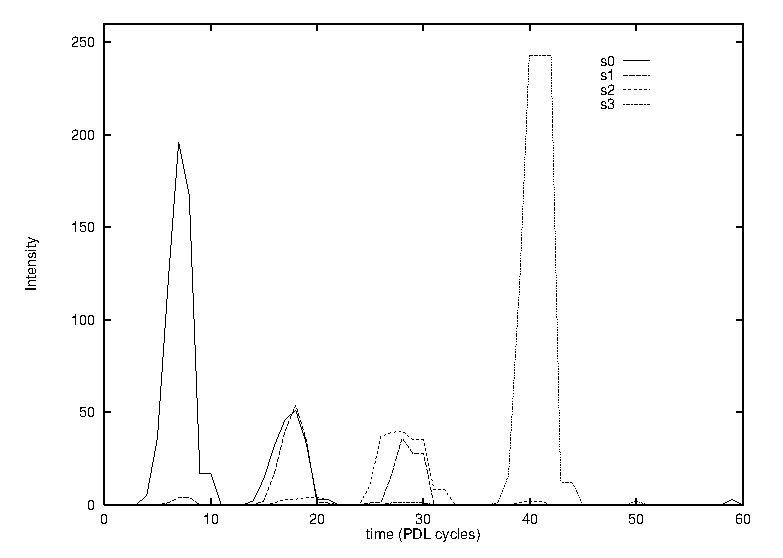
\includegraphics[width=9cm]{lang_games/region1.eps}}
\caption{The for noise filtered sensed view of robot $r0$ as seen in \figref{f:perception1}.}
\label{f:region1}
\end{figure}

What does a robot detect of a light source? From Figures~\ref{f:perception1} and~\ref{f:perception2} it becomes clear that the robots detect peaks of intensity of the sensory stimuli in contrast to some background noise. Applying the Hamilton function to \figref{f:perception1} results in \figref{f:region1}. Each region where the response is greater than zero will from now on be called a segment. It is assumed that each segment corresponds to a light source. Although in the original figure only 4 regions of interest were identified, the above method identifies 6 segments. The two additional segments come from small perturbations in the landscape that exceed the noise values a little bit. This does not necessarily mean that these perturbations cannot be due to noise, but it can also be due to reflection.

To filter out these segments, an additional rule is applied that a segment should contain more than one data point. Nevertheless, this will not guarantee that all irrelevant regions are filtered out. Neither are all relevant regions segmented. If two peaks (partly) coincide, this segmentation fails to extract the relevant segments. Nevertheless, as will be shown in subsequent chapters, the segmentation makes it possible to ground the sensing of the light sources.

The segmentation of the spatial view of \figref{f:perception2} does not recognise peak 4 (\tabref{t:perception2}), because the signal of sensory channel ${\bf s}_0$ does not decrease the noise value between peaks 3 and 4. Hence these two peaks are recognised as one segment.
\index{segmentation|)}

\subsubsection{Feature extraction}

\index{feature!extraction|(}
\index{feature!space}
\index{feature}
\index{feature!vector}

The segments that result from the segmentation have different lengths and may still have a lot of data. Therefore, it is desirable to describe each segment with one vector of low and {\em equal} dimension. Low dimension benefits computational efficiency. Equal dimension is used for consistency in the data, which makes the computations easier.

In line with pattern recognition and computer vision such a vector representation will be called a {\scshape feature vector} (see e.g. \citealt{fu:1976}). The elements of this feature vector will be called features. The extraction of the features is called feature extraction. The aim of the feature extraction is to extract features that bear {\em invariant} information about the light sources.

The feature extraction is applied to each segment $S_k$. It extracts for each sensory channel $i$ the value $\tau_{k,i,j}$ that has the highest value in $S_k$. Or, in other words, it gives the highest intensity of a sensory channel in the segment. But the absolute intensities have information about the distance of the light source, which is not an invariant property. Therefore, this highest value is normalised to the absolute highest value of all sensory channels in the segment. 

Formally the feature extraction of segment $S_k$ for sensory channel $i$ can be described by a function $\varphi({\bf s}_{k,i}):{\mathcal{S}} \rightarrow {\mathcal{S}'}$, where ${\mathcal{S}}=[0, 255]$ is the sensory channel space of some sensory channel and ${\mathcal S}'=[0, 1]$ is a one dimensional feature space.
\begin{eqnarray}
\varphi({\bf s}_{k,i}) = \frac{\max_{{\bf s}_{k,i}} (\tau_{k,i,l})}{\max_{S_k} (\max_{{\bf s}_{k,i}} (\tau_{k,i,l}))}
\label{e:sc-norm}
\end{eqnarray}

This function will yield a value 1 for the sensory channel on which the sensor reads the highest peak in a segment. For all other sensory channels the feature extraction yield a value between $[0, 1]$. Naturally, the values of these other features are irrelevant. However, this inference can easily be made by humans, but it should be unknown to the robots. This is so because in more complex environments this need not be an invariant property, and it is not the purpose to give the robots much knowledge. In addition, the so constructed invariance helps a human observer to analyse the experiments easier. 

The result of applying a feature extraction to the data of sensory channel $i$ will be called feature $f_i$, so $f_i=\varphi({\bf s}_{k,i})$. A feature thus designates a property of the sensed segment. In this case, the property can be described as the maximum intensity of a sensory channel in the segment relative to the maximum intensity of this segment. 

Segment $S_k$ can now be related to a feature vector ${\bf f}_k=(f_0,\ldots,f_{n-1})$, where $n$ is the total number of sensory channels. The space that spans all possible feature vectors ${\bf f}$ is called the $n$ dimensional feature space ${\mathcal F}={\mathcal S}^{'n}$, or feature space for short. Although this need not be so, in the current experiment the dimension of the feature space is equal to the number of sensory channels.


Applying the feature extraction of Equation \ref{e:sc-norm} to the sensing of \figref{f:region1} would result in the context given in \tabref{t:sc_relative}. Consider for example segment 1 of \figref{f:region1}. In this segment the top of sensory channel ${\bf s}_0$ has a value of 200, the top of ${\bf s}_1$ has value 4 and the two other sensory channels have values 0. Normalising the tops of this segment to the highest value yields $f_0=1.00$, $f_1=0.02$, $f_2=0.00$ and $f_3=0.00$ (cf. \tabref{t:sc_relative}).

\begin{table}
\centering
\begin{tabular}{crd{3}d{3}d{3}d{3}}
\lsptoprule
${\bf f}$ & \multicolumn{1}{c}{t} & \multicolumn{1}{c}{$f_0$} & \multicolumn{1}{c}{$f_1$} & \multicolumn{1}{c}{$f_2$} & \multicolumn{1}{c}{$f_3$}\\
\midrule
1 & 7 & 1.00 & 0.02 & 0.00 & 0.00\\
2 & 18 & 0.94 & 1.00 & 0.07 & 0.00\\
3 & 28 & 0.00 & 0.90 & 1.00 & 0.03\\
4 & 40 & 0.00 & 0.00 & 0.01 & 1.00\\
5 & 50 & 0.00 & 0.00 & 0.00 & 1.00\\
6 & 59 & 1.00 & 0.00 & 0.00 & 0.00\\
\lspbottomrule
\end{tabular}
\caption{Feature vectors ${\bf f}$ after applying the feature extraction measuring the relative intensity of a sensory channel in a given segment.}
\label{t:sc_relative}
\end{table}


The complete process of sensing and segmentation results in what is called the {\scshape context}.\index{context} This context $Cxt$ is a set of segments $S_i$ that relate to their feature vectors, so
\begin{eqnarray}
Cxt=\{S_0,\ldots,S_m\} \rightarrow \{{\bf f}_0,\ldots,{\bf f}_m\}
\end{eqnarray}
where $m$ is the context size.

The feature extraction that calculates the relative intensities is the only transformation used in the experiments reported here. In \citealt{steelsvogt:1997} and \citealt{vogt:1998b} the feature extraction function calculates the absolute peak values. Other functions have been introduced for categorising spatial categories as in \citealt{steels:1996d}. Still other functions have been designed for use in the Talking Heads experiments \citep{belpaeme:1998,steelskaplan:1999}. In the Talking Heads experiment as well as in this application, the functions were designed by hand. \citet{dejong:1999} and \citet{belpaeme:1999} have shown that such functions can be learned or evolved, respectively.\footnote{Note that Belpaeme calls the feature extraction function ``feature detectors''.}
\index{feature!extraction|)}

\subsection{Discrimination games}\label{s:cm:dg}\index{discrimination game|(}
In a language game each robot is interested in categorising one or more segments from the context they constructed. The speaker is interested in the segment which it wants to communicate and the hearer is interested in the segment(s) that the speaker can possibly communicate. The segment that the speaker wants to communicate is called the {\scshape topic}. For the hearer these segments are called the {\scshape potential topics}. For each (potential) topic the robots {\em individually} play a discrimination game.

As explained in \sectref{s:lg:perception}, a segment is related to a feature vector. This feature vector is a point in the feature space. The first step of the discrimination game is to categorise this feature vector with one or more categories that the robot has stored in its memory and that resemble this point in the feature space. A category is defined as some region in the feature space. A feature vector is categorised with that category for which the feature vector falls within that region.

\index{discrimination}
When the segments are categorised, the robots need to select the categories of the topic that are not used to categorise any other segment in the context. The process that does this is called {\scshape discrimination} (cf. \citealt{steels:1996b}). The discrimination can have different outcomes. If one or more categories are found, the discrimination is successful and hence the discrimination game is a success. In this case, the resulting categories can be used in the naming phase of the language game. If no distinctive category is found, this means that the repertoire of categories in the robot's memory is not sufficient to do the task.  At the start of each experiment, the repertoire of categories (or ontology) is empty. So, no categorisation can be found and hence no discrimination game can be successful. To overcome this problem in the future, the robot can expand its repertoire of categories.
\index{ontology}\index{distinctive category}

The complete task of categorisation, discrimination and adaptation is modelled by a discrimination game \citep{steels:1996b}. The basis of the model has not changed since its first introduction in 1996, but the implementation and precise details have been adjusted ever since. The first robot implementation of the model can be found in \citealt{steelsvogt:1997} and \citealt{vogt:1998a}. The model exploits a selectionist mechanism of generation and selection of categories. This results in the self-organisation of categories and has the properties of a dynamical system.

Different types of methods for representation in the discrimination game have been developed: the binary tree method \citep{steels:1996b}, the prototype method \citep{dejongvogt:1998,vogt:1998b} and the adaptive subspace method \citep{dejongvogt:1998,dejong:2000}. The prototype method and a variant of the adaptive subspace method, which will be called the binary subspace method are investigated in this book and shall be explained in this section. Before doing so, a more general description of the discrimination game model is presented.

Following \citet{steels:1996b}, the discrimination game can be defined formally as follows: Assume that the robots can relate their feature vectors to categories and suppose that the robots have categorised a set of categories $C_k=\{c_0,\ldots,c_{n-1}\}$ for the feature vectors relating to segment $S_k$. Let $S_t$ be the topic. The topic is the segment for which the robots try to find distinctive categories. A category is distinctive if it is related to the topic, but not to any other segment in the context $Cxt$. The distinctive categories are temporarily stored in a distinctive category set $DC$. If $DC \neq \emptyset$, the discrimination game is a success. $DC$ is passed to the naming game model that the robots use to communicate. If $DC=\emptyset$, the discrimination game fails and one or more new categories should be created. Consequently, there are three parts in the discrimination game:

\begin{enumerate}
\item The distinctive category set $DC$ is constructed according to the following relation: \begin{eqnarray}DC = \{c_i \in C_t \mid \forall S_k \in Cxt \backslash \{S_t\}: \neg c_i \in C_k\}\end{eqnarray}

\item If $DC \neq \emptyset$, the discrimination game is a success. Possibly adapt the scores of $c_i \in DC$ and pass the $DC$ to the naming game model.

\item If $DC = \emptyset$, then create a new category as ill be explained below.

\end{enumerate}

So, how are feature vectors categorised and how are categories created? The two models that do this are explained hereafter.\index{discrimination game|)}

\subsubsection{The prototype method}\label{s:cm:prototype}
\index{prototype|(}
\index{prototype!method|(}
\index{categorisation|(}
\index{category|(}

The prototype method is the main method investigated in this book. In this method the categories are defined in terms of prototypes. In the pattern recognition literature, (see e.g. \citealt{banks:1990}), a {\scshape prototype} is defined as ``a single representative sample'' in the feature space, i.e. as a point in the feature space. However, a category is defined as a {\scshape region} in the feature space. For a prototype, this region can be defined by those points in the feature space that are nearest to this prototype. Therefore, a prototypical category can be defined as a region in the feature space that is represented by a prototype.

The prototypical categories are represented by prototypes and some scores: $c=\langle {\bf c},\nu,\rho,\kappa \rangle$, where ${\bf c}=(x_0,\ldots,x_{n-1})$ is a prototype in the $n$ dimensional feature space, and $\nu$, $\rho$ and $\kappa$ are some scores. As mentioned, categorisation is the process of finding categories for which the feature vector lies within the region that is defined by the category. The categorisation of this is done with the 1-nearest neighbour algorithm. The 1-nearest neighbour algorithm returns the prototype that is nearest to observed feature vector. \index{k-nearest neighbour algorithm}\index{category!prototypical}

\index{feature!space}
It can be useful to define categories at different levels of generality or specificity. If two segments are very distinctive, i.e. the distance between them in the feature space is large, then these segments can be categorised using general categories. However, if the two segments are relatively close to each other in the feature space, the categories may need to be more specific. This means that the regions should be smaller. When sensing a referent under different circumstances in different language games, the extracted feature vectors of the segmented segments differ as well. To select the categories as consistent as possible for various feature vectors relating to some referent in different language games, a general category is most useful. The region of a general category is larger, thus enhancing the chance that different segments of a referent from different language games is represented with the same categories. To enable discrimination under these different conditions and allowing both generality and specificity the categories are constructed in different versions of the feature space.\footnote{Note that the term ``specificity'' is defined differently in the next chapter. There it is defined as a measure that indicates how well a robot names a referent. Here ``specificity'' is used in the more intuitive and common sense.} Each version has an increasing resolution of the feature space.

If the discrimination game is a failure, the ontology has to be expanded. Some new prototypes will be constructed and stored in the robot's memory. It is done by exploiting one arbitrary dimension (or feature) of the feature vector in one of the versions of the feature space. Suppose there are versions of the feature space ${\mathcal F}_\lambda$, where each $\lambda$ designates the resolution of the feature space. In each dimension of the feature space ${\mathcal F}_\lambda$ there are a maximum of $3^\lambda$ exploitations, where $\lambda=0,1,2,\ldots$~. The choice of 3 is more or less arbitrary, but should not be too large. 

Suppose that in the discrimination game the robot tried to categorise feature vector ${\bf f}=(f_0,\ldots,f_n)$. New categories are created now as follows:

\begin{enumerate}

\item Select an arbitrary feature $f_i>0$.

\item Select the feature space ${\mathcal F}_\lambda$ that has not yet been exploited $3^\lambda$ times in dimension $i$ for $\lambda$ as low as possible.

\item Create new prototypes ${\bf c}_j = (x_0,\ldots,x_{n-1})$ where $x_i=f_i$ and the other $x_r$ are made of already existing prototypes in ${\mathcal F}_\lambda$.

\item Add the new prototypical category $c_j=\langle {\bf c}_j,\nu_j,\rho_j,\kappa_j \rangle$ to the feature space ${\mathcal F}_\lambda$. $\nu_j$ is a category score that indicates the effect of discrimination. $\rho_j$ is the effectiveness score that indicates the use of the category in the language game. $\kappa_j$ indicates how general the category is. The initial values of $\nu_j$ and $\rho_j$ are set to 0.01. $\kappa_j$ is a constant, which is calculated as in equation \ref{e:lg:kappa}. \index{category!prototypical}

\end{enumerate}


The reason to exploit only one feature of the topic, rather than to exploit the complete feature vector of the topic is to speed up the construction of categories. The scores are introduced to enable a better selection in the naming game and are updated after a discrimination game ($\nu$) or a naming game ($\rho$) as follows:\index{score}\index{score!categorisation}

\begin{itemize}
\item The categorisation score $\nu$ is used to indicate how often the category is used to distinctively categorise a feature vector. It is calculated according to the following equation:
\begin{eqnarray}
\nu = \nu + \eta \cdot X
\label{e:lg:nu}
\end{eqnarray}
where
\begin{eqnarray}
X = \left \{ \begin{array}{rl}
1 & \mbox{if categorised distinctive}\\\nonumber
0 & \mbox{if categorised, but not distinctive}\nonumber
\end{array} \right.
\end{eqnarray}
where $\eta$ is a learning rate. The default value of the learning rate is set to $\eta=0.99$.
\index{score!effectiveness} \item The effectiveness score $\rho$ is used to indicate the effective use in the language. I.e.
\begin{eqnarray}
\rho = \rho + \eta \cdot Y
\label{e:lg:rho}
\end{eqnarray}
where
\begin{eqnarray}
Y = \left \{ \begin{array}{rl}
1 & \mbox{if used in language game}\\\nonumber
0 & \mbox{if distinctive, but not used in language game}\nonumber
\end{array} \right.
\end{eqnarray}
where $\eta$ is the learning rate.
\item Another score that is calculated is the depth score $\kappa$. It indicates how general the category is. As mentioned, if possible it is preferable to use categories that are as general as possible. A category is as general as possible if it is in a feature space ${\mathcal S}_\lambda'$ with $\lambda$ as small as possible. Because of the resolution of the sensors, the resolution cannot increase in a feature space with $\lambda=5$, so that is the most specific feature space.\index{score!depth}
\begin{eqnarray}
\displaystyle
\kappa_M=1 - \frac{\lambda}{5}
\label{e:lg:kappa}
\end{eqnarray}
\noindent
This score implements a preference for the most general category, which is conform  with \citealt{steels:1996b}. 

\index{score!meaning}\index{meaning}
\item In the naming game, the three scores are taken together to form a meaning score $\mu$. Note that it is allowed to talk about meaning, since this score is only evaluated in relation to a form.
\begin{eqnarray}
\displaystyle
\mu=\frac{1}{3}\cdot (\nu+\rho+\kappa)
\end{eqnarray}
\noindent
The value of $\mu$ is averaged so that it can be scaled separately when using it in the naming phase as will be explained in the next section.
\end{itemize}


Because once the scores $\nu$ and $\rho$ become greater than zero, they will never become zero again, they can by way of updating (equations \ref{e:lg:nu} and \ref{e:lg:rho}) only approach zero asymptotically. In order to give new categories a chance to be selected, their initial values are not set to 0, but to 0.01.

There is another adaptation that is done with a prototypical category when it has been successfully discriminated. If the category is used as the meaning in a language game successfully, i.e. it has been the subject of a successful communication, the prototype of the category is shifted towards the feature vector that it categorises according to equation \ref{eq:3.9}:
\begin{eqnarray} \label{eq:3.9}
{\bf c}_3' = {\bf c}_3 + \epsilon \cdot ({\bf f}_t - {\bf c}_3)
\end{eqnarray}
where ${\bf c}_3'$ is the new vector representation of  ${\bf c}_3$ after shifting this category with a step size of $\epsilon$ towards ${\bf f}_t$. In the experiments $\epsilon=0.1$. This way the prototypical category becomes a more representative sample of the feature vector it categorised.

Because the resolution of a sensor is limited to six feature spaces, ${\mathcal F}_0$ to ${\mathcal F}_5$ are the only ones available. Another reason to keep the number of feature spaces limited is to keep the computational efficiency within limits. Besides, as will become clear in the experiments, ${\mathcal F}_1$ will usually be sufficient to discriminate.
\index{feature!space}

The prototype method is a variant of an instance-based learning technique (see e.g. \citealt{ahaetal:1991,mitchell:1997}). As mentioned, it uses the $k$-nearest neighbour algorithm, where $k=1$. Instance-based learning assumes a set of training examples (prototypes) that consists of both positive and negative examples of some categorisation. However, in the prototype method training examples are added to the feature space when a categorisation failed. The validation of a positive or negative example is based on the discriminative power of the categorised prototype. The adaptation of scores that help to select the distinctive categories in the naming phase is very much like the update of $Q$ values in reinforcement learning (see e.g. \citealt{suttonbarto:1998}). \index{instance-based learning}\index{reinforcement learning}

\subsubsection{An example}

The prototype method can be illustrated with an example. Suppose there is an ontology of prototypes on ${\mathcal F}_0$ and ${\mathcal F}_1$ as displayed in \figref{f:lg:proto} (a) and (b). In Figure (a) there is one prototype ${\bf c}_0=(0.20,0.90)$. In Figure (b) there are two prototypes ${\bf c}_1=(0.25,0.75)$ and ${\bf c}_2=(0.65,0.75)$. Left of the division line in the space is category ${\bf c}_1$ and right is category ${\bf c}_2$. Suppose the robot has related topic $t$ with a feature vector ${\bf f}_t=(0.30,0.10)$ and it has another segment $s$ in its context related with feature vector ${\bf f}_s=(0.15,0.80)$.\footnote{Note that these vectors are made up to illustrate the example.} Then both ${\bf f}_t$ and ${\bf f}_s$ are categorised with $\{{\bf c}_0,{\bf c}_1\}$. Hence the categorisation of topic $t$ is not distinctive. So, the ontology has to be expanded. 

\begin{figure}
\centering
\subfigure[${\mathcal F}_0$]{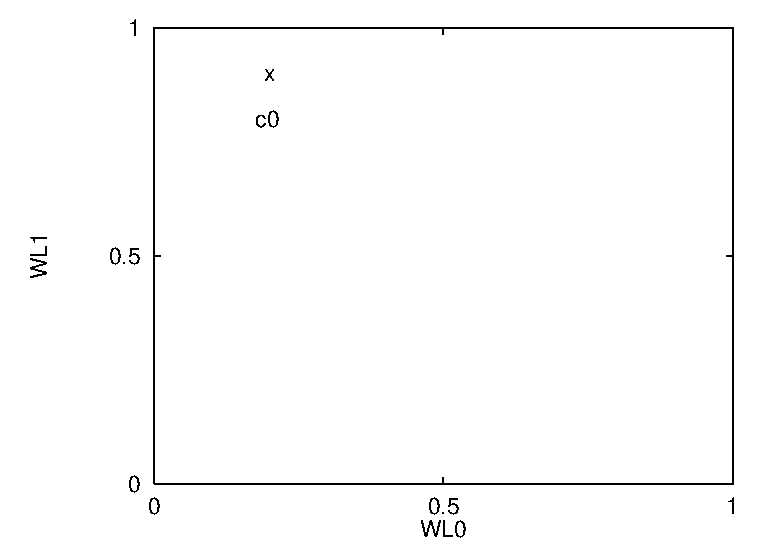
\includegraphics[width=5.5cm]{lang_games/proto0.eps}}
\subfigure[${\mathcal F}_1$ - i]{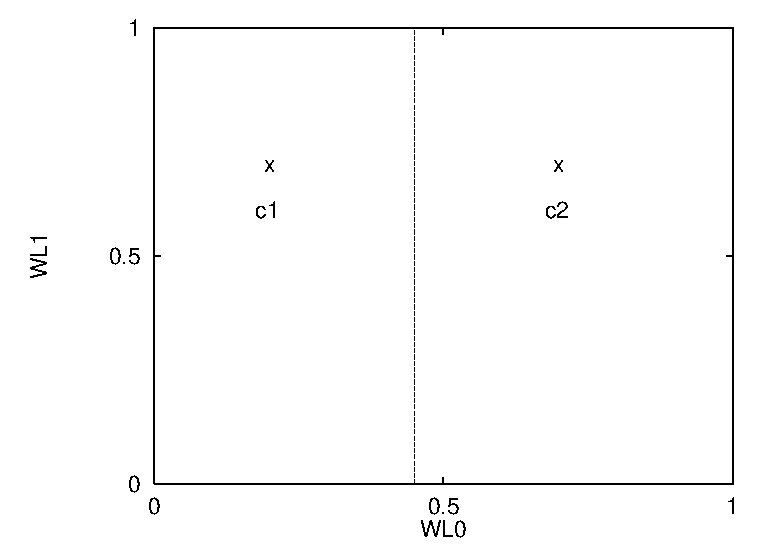
\includegraphics[width=5.5cm]{lang_games/proto1.eps}}
\subfigure[${\mathcal F}_1$ - ii]{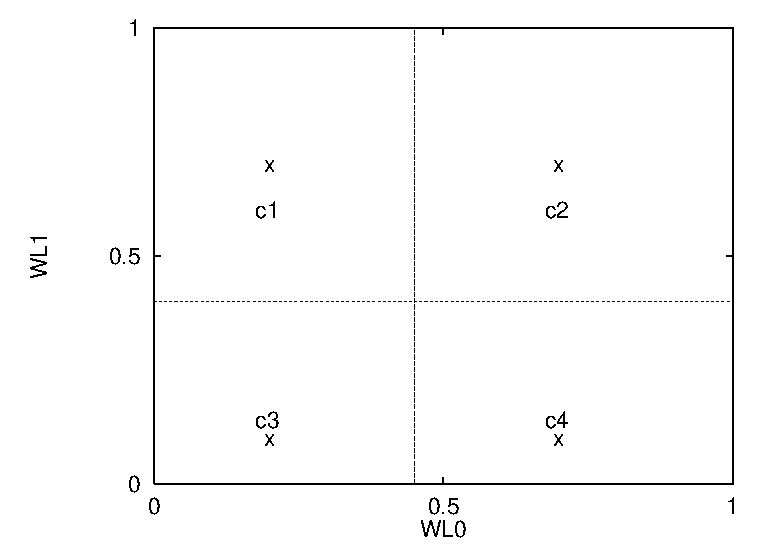
\includegraphics[width=5.5cm]{lang_games/proto1a.eps}}
\subfigure[${\mathcal F}_1$ - iii]{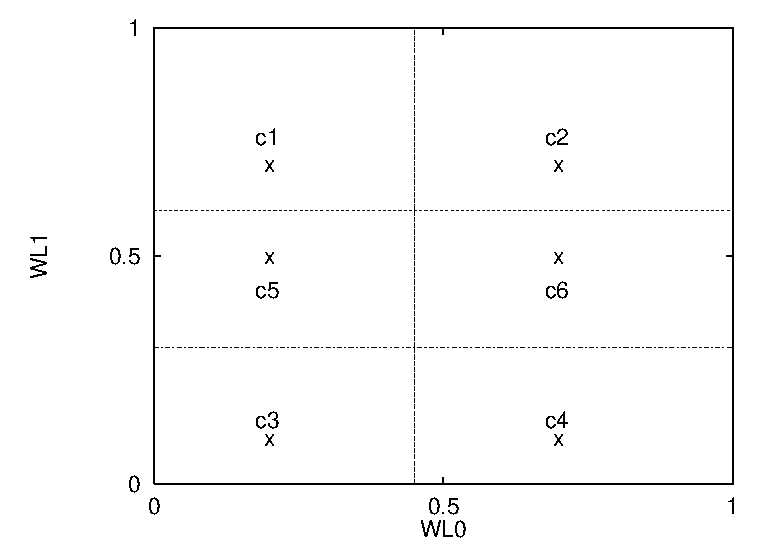
\includegraphics[width=5.5cm]{lang_games/proto2.eps}}
\caption{These figures show feature spaces ${\mathcal F}_0$ (a) and ${\mathcal F}_1$ (b), (c) and (d), each with their prototypes (x) as used in the example. The figures are displayed in two dimensions for illustrative purposes; in the actual implementation the spaces have 4 dimensions.}
\label{f:lg:proto}
\end{figure}

The robot selects one dimension of the feature space to exploit. Suppose this is dimension {\scshape wl}\oldstylenums{1}. In this dimension, the topic has a feature with value 0.10. The robot has to select a feature space on which there is still place in the selected dimension. In ${\mathcal F}_0$ each dimension can be exploited $3^0=1$ time. This has already happened, so the robot checks if it can exploit the next space, ${\mathcal F}_1$. In this space each dimension can be exploited $3^1=3$ times. Dimension {\scshape wl}\oldstylenums{1} has only been exploited once, so this dimension can still be exploited. New prototypes are constructed with the points $(x,0.10)$, where $x$ is filled in with the corresponding co-ordinates of the already existing prototypes. If some dimensions are not exploited yet, the new prototypes will not become active until all dimensions of the feature space are exploited. This yields two new prototypes ${\bf c}_3=(0.25,0.10)$ and ${\bf c}_4=(0.65,0.10)$, see \figref{f:lg:proto} (c). Since each dimension of ${\mathcal F}_1$ can be exploited up to 3 times, the robot can exploit each dimension of this space only once more. This has been done for one dimension in \figref{f:lg:proto} (d).

\index{distinctive category}
When the robot needs to find distinctive categories in this new ontology based on the same feature vectors as before, ${\bf f}_t$ will be categorised with $\{{\bf c}_0,{\bf c}_3\}$ and ${\bf f}_s$ with $\{{\bf c}_0,{\bf c}_1\}$. Yielding distinctive category set $DS=\{{\bf c}_3\}$. Now ${\bf c}_3$ may be used in the language game as the meaning of the symbol that is communicated. If this is done successfully, the category is shifted in the direction of the observation by using the following equation (see Equation \ref{eq:3.9}):\index{meaning}
\[
{\bf c}_3' = {\bf c}_3 + \epsilon \cdot ({\bf f}_t - {\bf c}_3)
\]
so, in this case, ${\bf c}_3'=(0.255,0.3)$.

\begin{figure}
\centerline{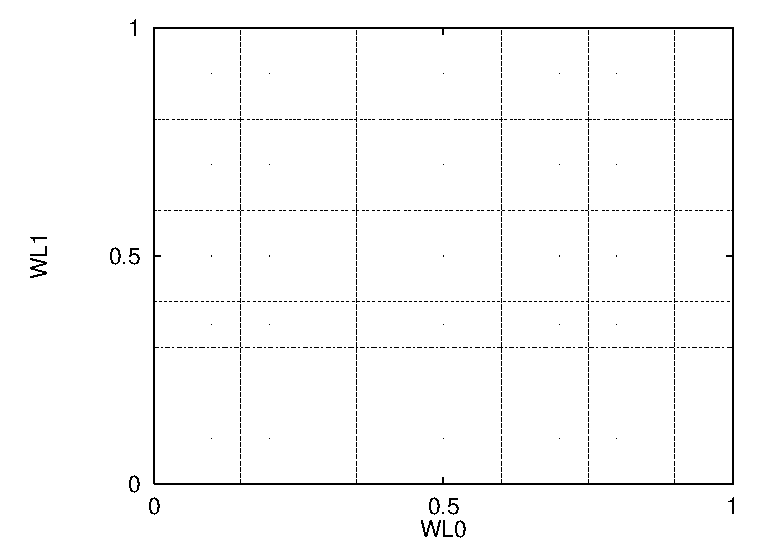
\includegraphics[width=9cm]{lang_games/proto3.eps}}
\caption{A possible feature space ${\mathcal F}_2$. In this space each dimension may be exploited up to 9 times. Again for illustrative purposes the space is shown in 2 dimensions. Note that the prototypes here are displayed as small points.}
\label{f:lg:proto2}
\end{figure}


\figref{f:lg:proto2} shows a 2 dimensional version of a possible feature space ${\mathcal F}_2$. There are an increasing number of categories possible at each increasing ``layer''. In feature space ${\mathcal F}_0$ there is one place per dimension to be exploited, in ${\mathcal F}_1$ there are 3 places etc. So, ${\mathcal F}_0$ has a maximum of 1 prototype, ${\mathcal F}_1$ has a maximum of $3^4=81$ prototypes (recall there are 4 dimensions), in ${\mathcal F}_2$ there are $9^4=6561$ possible prototypes, etc. 

\index{prototype!method|)}
\index{prototype|)}

\subsubsection{Binary subspace method}\label{s:cm:binary}
\index{binary!subspace method|(}
\index{binary!subspace|(}

The prototype method will be compared with the binary subspace method. The binary subspace method makes use of another way to make categorical distinctions. It is based on the original model introduced by Luc \citet{steels:1996b} that has previously been implemented on the mobile robots \citep{steelsvogt:1997,vogt:1998a}. In the original model categories are constructed from trees that make binary divisions of only one dimension of the feature space. The categories that are constructed may have one dimension, but can also be a conjunction of more dimensions. Hence they do not necessarily cover the $n$ dimensions of the feature space. \figref{f:lg:binarytree} shows how the trees are constructed.

\index{binary!tree method}

\begin{figure}[t]
\centerline{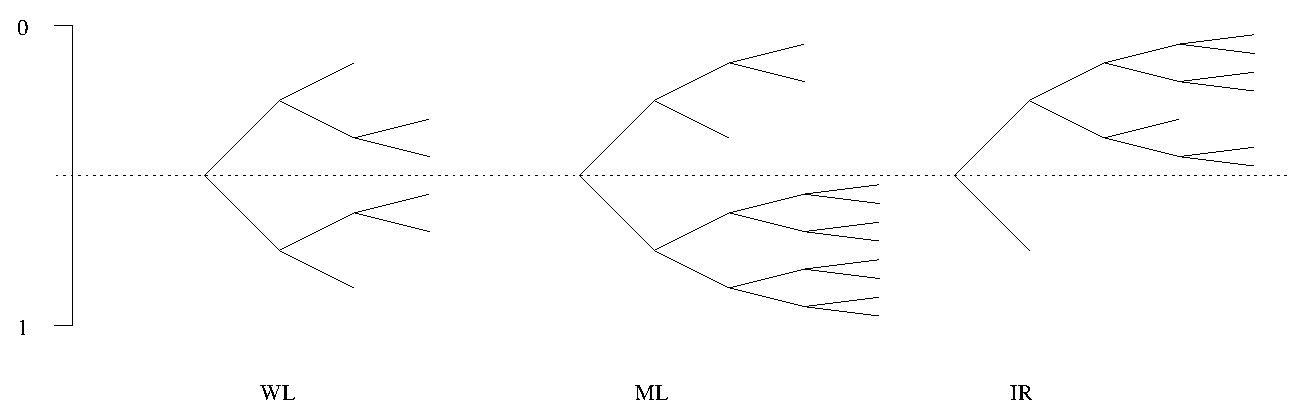
\includegraphics[width=\textwidth]{discr_games/binary_tree.eps}}
\caption{Categories represented as binary trees. Every sensory channel (like {\scshape wl}, {\scshape ml} and {\scshape ir}) is associated with a category tree. The root node of the tree is sensitive to whole range of the sensory channel. The tree is incrementally constructed during the evolution of discrimination games. Every time the discrimination game fails, two new nodes may be constructed by splitting one node.}
\label{f:lg:binarytree}
\end{figure}

The binary subspace method combines the binary tree method with the adaptive subspace method \citep{dejongvogt:1998,dejong:2000}. In the adaptive subspace method, the categories (or subspaces) are always in the $n$ dimensions of the feature space. In the binary subspace method, the co-ordinates of a feature space ${\mathcal F}_\lambda$ are splitted in one dimension at a time. When all dimensions are thus exploited, the first categories at this space are born.

Categorisation in the subspace is done by relating feature vectors to those subspaces in which the feature vectors fall.


A subspace is defined as an $n$ dimensional rectangle that is surrounded by their boundaries in each dimension of the feature space ${\mathcal F}_\lambda$. Note that this shape of a subspace differs from the one introduced by \citet{oja:83}. Suppose there is a lower boundary $x_i$ and an upper boundary $y_i$ in dimension $i$ of ${\mathcal F}_\lambda$. These boundaries do not necessarily coincide with the boundaries of ${\mathcal F}_\lambda$. A category $c_j$ can be defined by these boundaries in each dimension of ${\mathcal F}_\lambda$: $c_j=\langle x_0, y_0, \ldots, x_{n-1}, y_{n-1}, \nu_j, \rho_j, \kappa_j \rangle$ for $n$ dimensions. Like for the prototype method, $\nu_j,\rho_j$ and $\kappa_j$ are scores.

A feature vector ${\bf f}=(f_0,\ldots,f_{n-1})$ can be categorised with category $c_j$ if $x_i < f_i \leq y_i$ for all dimensions of the feature space.

At the start of the experiment the category of ${\mathcal F}_0$ is given. This category spans the complete feature space. When a discrimination game fails, new categories should be formed. This is done by exploiting only one dimension every time the game fails. The following list describes how this is done step by step. Suppose that ${\bf f}$ is the feature vector that has been the topic of the discrimination game.

\begin{enumerate}
\item Select the category $c=\langle x_0,y_0,\ldots,x_{n-1},y_{n-1},\nu,\rho,\kappa \rangle$ that categorised ${\bf f}$ in the feature space ${\mathcal F}_\lambda$ for which $\lambda$ is greatest. This means that no categorisation is made in ${\mathcal F}_{\lambda+1}$.

\item Select a dimension $i$ of $c$ that has not been exploited yet in feature space ${\mathcal F}_{\lambda+1}$ and for which $f_i>0$.

\item Create the following lower and upper boundaries: $x_i'=x_i$, $y_i'=x_i+\frac{1}{2} \cdot (y_i-x_i)$, $x_i''=x_i+\frac{1}{2} \cdot (y_i-x_i)$ and $y_i''=y_i$.

\item If there are lower and upper boundaries $x_p^r$ and $y_p^r$ for some $r$ in all other dimensions $p$ of feature space ${\mathcal F}_{\lambda+1}$, then construct new categories by combining all these lower and upper boundaries and adding scores. This yields categories like $c_q = \langle x_0^r,y_0^r,\ldots,x_{n-1}^k,y_{n-1}^k,\nu_q,\rho_q,\kappa_q \rangle$.

\item If there are no lower and upper boundaries in all other dimensions, then add $x_i',y_i',x_i'',y_i''$ to the set of lower and upper boundaries in ${\mathcal F}_{\lambda+1}$.

\end{enumerate}

The binary subspace method differs from the binary tree method of \citet{steels:1996b} in that a category covers all the $n$ dimensions of the feature space. Steels defines categories in 1 to $n$ dimensions, by taking conjunctions of the nodes in the binary trees. Conjunctions can have nodes at different hierarchical layers. Processing all these possible categories is computationally very costly. Suppose there are six hierarchical layers in the tree (as in the prototype method, the binary subspace method has six feature spaces) and 4 dimensions, which is completely filled. Then there are $6\cdot 4=24$ one-dimensional categories. There are $6^2\cdot 2!=216$ two-dimensional categories. There are $6^3\cdot 2!=432$ three-dimensional categories and $6^4=1296$ four-dimensional categories. This makes a total of 1968 possible categories to be explored. The binary subspace method only considers $n$ dimensional conjunctions of nodes each layered at the same layer in the tree. This yields a maximum of only 6 categories to be explored.

\index{adaptive subspace method}\index{De Jong, Edwin}
The adaptive subspace method developed by Edwin De Jong also differs from the binary subspace method \citep{dejongvogt:1998,dejong:2000}. Like in the binary subspace method, De Jong splits a category from feature space ${\mathcal F}_\lambda$ in ${\mathcal F}_{\lambda}$ very similar to the binary subspace. However, De Jong's agents directly create a new category, which is the former category splitted in one dimension. Every time this is done, only two new categories are made. In the binary subspace method, more categories may be made. Another difference is that De Jong lets his agents do not create new categories every time the discrimination game fails, but it is done after a fixed number of failures. The choice which subspace is splitted and in which dimension is calculated from some statistics of previous failures to find distinctions. For a detailed explanation of the adaptive subspace method see \citealt{dejongvogt:1998} and \citealt{dejong:2000}.

\begin{figure}
\centering
\subfigure[${\mathcal F}_0$]{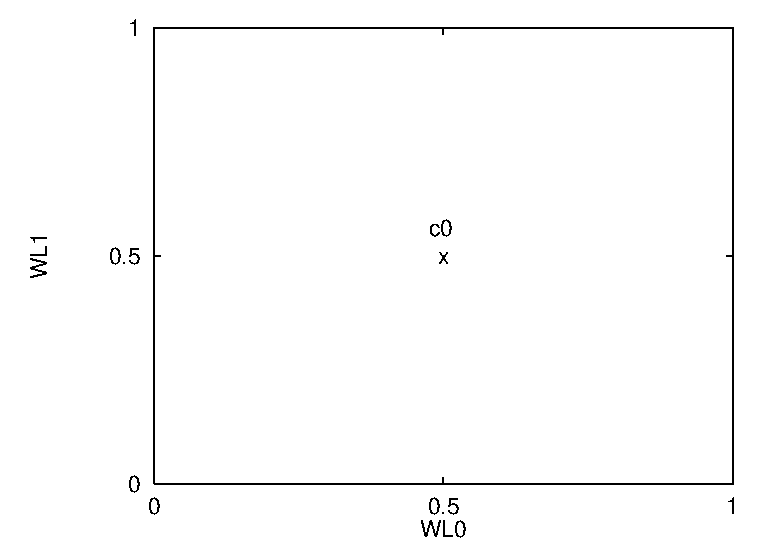
\includegraphics[width=5.5cm]{lang_games/binary0.eps}}
\subfigure[${\mathcal F}_1$]{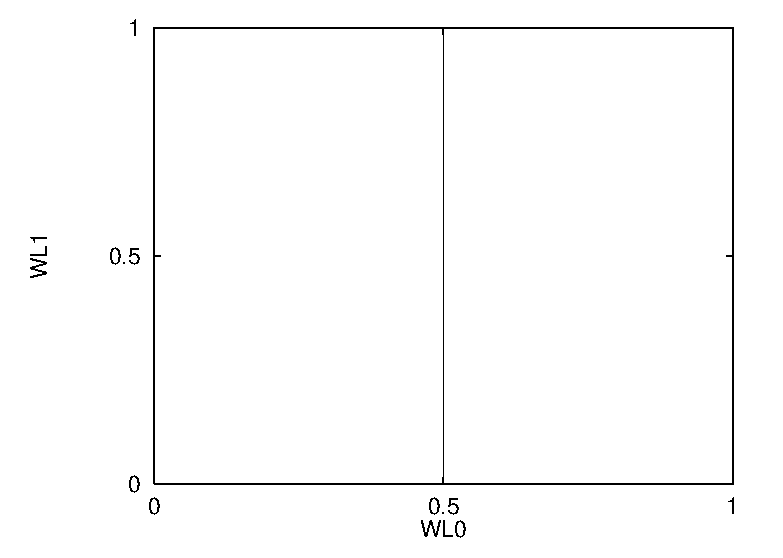
\includegraphics[width=5.5cm]{lang_games/binary1.eps}}\\
\subfigure[${\mathcal F}_1$]{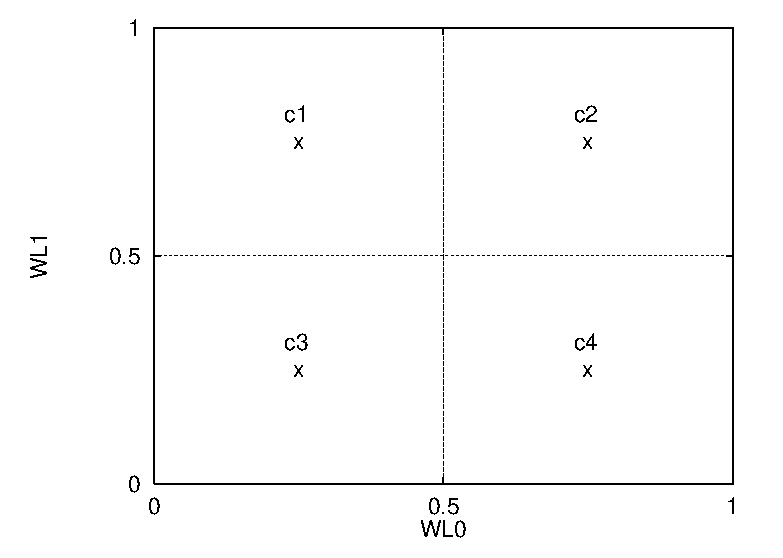
\includegraphics[width=5.5cm]{lang_games/binary1a.eps}}
\subfigure[${\mathcal F}_2$]{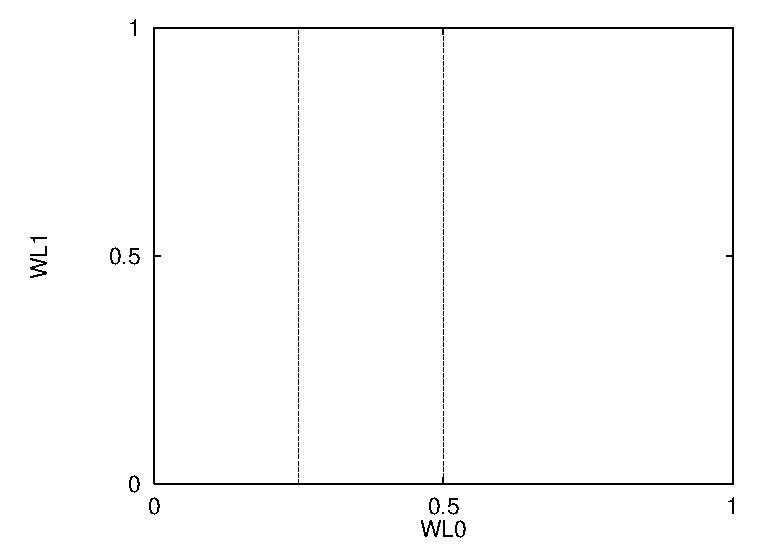
\includegraphics[width=5.5cm]{lang_games/binary2.eps}}\\
\subfigure[${\mathcal F}_2$]{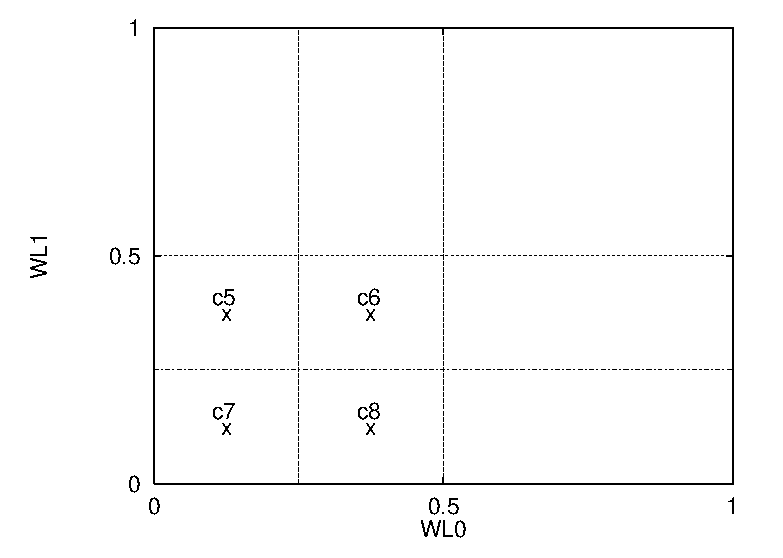
\includegraphics[width=5.5cm]{lang_games/binary2a.eps}}
\caption{The binary subspace method splits the feature space at the lower layer (i.e. $\lambda$ is smaller) in each dimension at a time. The split divides the former subspace in two equal halves in one dimension. As the plot in Figure (b) did for $c_0$ in Figure (a). A category is not formed until each dimension is exploited. If another split is made as in Figure (c), new categories are formed. Figures (d) and (e) are two subsequent splits of category $c_3$ from Figure (c). The last split results in four new categories on ${\mathcal F}_2$. If a split would be made on $c_1$ in dimension {\scshape wl}\oldstylenums{1} of Figure (c). Again four new categories are constructed.}
\label{f:lg:subspace}
\end{figure}

Unlike in the prototype method, once a category is made, it is static, i.e. it does not shift in the feature space. Like the categories of the prototype method, the binary subspaces are associated with some scores. These scores are the same as for the prototype method. 

One major difference of the binary tree, binary subspace and adaptive subspace with the prototype method is that there is not necessarily a categorisation in each feature space ${\mathcal F}_\lambda$ where there are categories. In the prototype method, the entire space is always covered once a category is there. This is not the case in the other methods. 

A more fundamental difference with the prototype method is that the binary subspace method, like the binary tree method and the adaptive subspace method is biologically less plausible. Humans do not make binary distinctions of the world. The feature space of observations is usually not divided in binary distinctions.

The binary subspace method, like the adaptive subspace method \citep{dejong:2000} is a type of {\scshape adaptive resolution} generalisation. In these methods a multidimensional space is divided in subregions based on some criteria in order to solve some tasks. Examples of such learning techniques can be found in \citealt{chapmankaebling:1991} and \citealt{moore:1995}.
\index{binary!subspace method|)}
\index{binary!subspace|)}
\index{category|)}
\index{categorisation|)}

\subsubsection{Summary}

In this section the discrimination game model has been introduced. The aim of a discrimination game is to find distinctive categories that categorise one or more segments. Categories can be defined differently. In this book two methods are compared. The prototype method defines a prototype as a point in the feature space and a category is then defined as the region in the space where the points are closest to the prototype. The binary subspace method defines a category as a subspace that is constructed by splitting another space in two equal halves at one dimension. Categories are structured in different versions of the feature space, where each version has a different resolution. This allows making distinctions that are more general or more specific. 

The prototype method is used in almost all experiments. In one experiment the binary tree method is used, and in still another experiment a fuzzy approach of the prototype method is used. This latter method is explained in \chapref{ch:cat}.

The feature vector that relates to the topic is categorised with a category that covers the feature vector. A category is distinctive if it is not related to any other feature vector in the context than to the topic. If distinctive categories can be found, the discrimination game is a success. In this case the distinctive categories may be adapted, e.g. by shifting them, and one of the categories can be used as the meaning in the naming phase. If the discrimination game is a failure, new categories can be constructed.

\subsection{Lexicon formation}\label{s:cm:ng}

Now that each robot has categorised the (potential) topic(s) distinctively, they can communicate these distinctive categorisations. Communication is established by the speaker and hearer. The speaker names the category. The hearer tries to interpret this name, i.e. it tries to identify the uttered word-form so that it corresponds to the categorisation of the topic. The topic is supposed to relate to the referent that the speaker's utterance stands for. 

In some experiments the hearer already knows which topic this is prior to the verbal communication. This means that there is some sort of joint attention on the topic. This knowledge is exchanged from the speaker by means of extra-linguistic communication. In other experiments the hearer does not know yet what the topic is. The hearer then only has the uttered word-form and the distinctive categories at its disposal. The availability of such information is a source of discussions in the psycholinguistic literature (see e.g. \citealt{barrett:1995}) and the discussion in \chapref{ch:intro}. Therefore it is interesting to investigate whether and under what circumstances the robots can deal with these different types of knowledge.

When the hearer interpreted the utterance, the language game is successful when both robots communicated about the same referent. In case where the hearer already had this knowledge at its disposal, this is the case. Otherwise, the robots may evaluate whether they did so. This evaluation is called {\scshape feedback}. The evaluation of feedback is, like joint attention, done by means of extra-linguistic communication. Again, the availability of feedback to a language learner is of much debate in the psycholinguistic literature (see e.g. \citealt{bowerman:1988}). So, is this really necessary? 

Both types of extra-linguistic information is subject of investigation of this book. For this reason different types of language games have been developed: the ostensive game, guessing game, observational game and {\scshape xsl} game.

When the experiments start, however, the robots have no language to their disposal yet. They have to construct this. In the experiments the question of how grammar is evolved is left aside and only a lexicon is developed. How are forms associated with meanings? And how can both robots acquire a shared lexicon? To model this, the robots can adapt their lexicons. This lexicon development is based on the three mechanisms that Luc \citet{steels:1996a} proposed for lexicon formation: individual adaptation, cultural evolution and self-organisation.

The previous section presented the discrimination game model by which the first two steps (iconisation and discrimination) of the grounding problem is tackled. The model tries to find categories that relate to the topic, but not to any other segment that has been observed in that context. Such a category can be related to a form. If this is done, the category functions as the meaning of a semiotic sign in the Peircean sense. When this form is either arbitrary or conventionalised (e.g. through language) the sign becomes a symbol according to Peirce (see e.g. \citealt{chandler:1994}). Since it is assumed that meaning co-evolves with language (\chapref{ch:intro}), the symbol is grounded in language and hence the form will be conventionalised. The naming game model implements how the form is conventionalised.\index{category}\index{meaning}\index{Peirce, C.S.}\index{semiotics}\index{symbol}

\index{Steels, Luc}\index{naming game|(}
The lexicon formation is based on the naming game model introduced by Luc \citet{steels:1996a}. The naming game implements the communication between two agents that try to name the meaning of the referents they sensed in their environment. One of the agents plays the role of the speaker and chooses a topic from the segments that constitute the context. It searches its lexicon for a form-meaning association of which the meaning matches the category of the topic. The associated form is ``uttered'' and in turn, the hearer tries to understand the utterance. The hearer does so by searching its own lexicon for a form-meaning association of which the form matches the utterance. If there exist such an element, the hearer compares the associated meaning(s) with the category of the topic. If there is a match and both the speaker and the hearer named the same topic, the naming game is successful. Otherwise there is a failure. According to the outcome of the game the lexicon will be adapted. 

\subsubsection{Different language games}

One of the issues that will be investigated in this book is what type of extra-linguistic information is necessary to guide a meaningful lexicon formation. As mentioned above and in \chapref{ch:intro}, it is not clear what extra-linguistic information infants have at their disposal when learning language. Do they establish joint attention prior to the verbal communication? Or do they receive feedback on the effect of a linguistic interaction? Or is neither at their disposal? 

To investigate whether robots can develop a shared lexicon under these different circumstances, four types of language games have been implemented. In these language games different configurations of the availability of joint attention and feedback have been implemented as shown in \tabref{t:cm:games}. The different games can be summarised as follows:

\begin{description}
\item[Ostensive game] This game is conform with the original naming game model \citep{steels:1996a}. The speaker informs the hearer prior to the linguistic communication what the topic is, e.g. by means of pointing at the referent. Hence joint attention is established. It then produces a (linguistic) utterance, which the hearer tries to understand. Feedback is evaluated to check if both robots finally identified the same topic. This game has also been implemented in \citealt{steelsvogt:1997}.
\index{ostensive game}\index{joint attention}

\item[Guessing game] In the guessing game \citep{steelskaplan:1999}, the speaker does not provide the hearer with topic information. It produces an utterance and the hearer has to {\em guess} which referent the speaker is naming. As in the ostensive game feedback is evaluated to check if both robots finally identified the same topic. The guessing game has first been implemented in \citealt{vogt:1998c} and will be the model of most experiments in this book.
\index{guessing game}\index{feedback}

\item[Observational game] This game is influenced by the work of Mike \citet{oliphant:1997}. First joint attention is established, so the hearer knows in advance which segment is the topic. Access to this kind of information is what Oliphant calls ``observation''. The speaker produces an utterance, which the hearer tries to interpret. No feedback on the game's effect is evaluated, so the lexicon is adapted independent of the effectiveness of the game.
\index{observational game}

\item[XSL game] The {\scshape xsl} game is to check if either joint attention or feedback is really necessary. It is to show that lexicon formation does not work without joint attention of feedback. So, without providing topic information, the speaker produces an utterance. The hearer tries to interpret the utterance. The robots adapt their lexicons despite the fact that they have no idea what the other has been communicating. Note that {\scshape xsl} stands for ``cross-situational learning'' \citep{pinker:1989,siskind:1996}, which is the learning mechanisms on which this model is based. (As noted in the preface, this was not noted at the time of writing this book, so no further reference to the literature of cross-situational learning is made.)
\index{XSL game}
\end{description}

\begin{table}
\centering
\begin{tabular}{lcc}
\lsptoprule
Game & Joint attention & Feedback\\
\midrule
ostensive & Yes & Yes\\
guessing & No & Yes\\
observational & Yes & No\\
{\scshape xsl} & No & No\\
\lspbottomrule
\end{tabular}
\caption{A schematic overview of the extra-linguistic information that is available in the different language games.}
\label{t:cm:games}
\end{table}


The four games differ in the availability of joint attention and feedback as illustrated in \tabref{t:cm:games}. In most of the experiments reported in this book the guessing game is applied. The remainder of this section explains the different subparts of the naming: joint attention, production, understanding, feedback and adaptation.

\subsubsection{The lexicon}

Each agent constructs a lexicon. How does the lexicon look like? A lexicon is a set of form-meaning associations that an individual robot stores in its memory. The lexicons of the two robots in the experiments can differ and are shared when the lexical entries are used such that both robots can communicate a referent successfully. So, the lexicon consists of elements of form-meaning associations. Each form-meaning association $FM$ is a tuple of a form $F$, a meaning $M$ and an association score $\sigma$. So, the lexicon $L$ can be defined as:\index{lexicon}\index{form-meaning association}\index{lexicon}
\begin{eqnarray}
L=\{{\bf \mbox{FM}}_0, \ldots, {\bf \mbox{FM}}_N\}
\end{eqnarray}
\noindent
where $N$ is the size of $L$ and form-meaning ${FM}_i=\langle W_i,M_i,\sigma_i\rangle$. At the beginning of an experiment, $L=\emptyset$. It is constructed during the experiment. The form $F$ is an arbitrary string of characters from the alphabet. The shape of a form is given as a ``{\scshape cvcv}'' string where {\scshape c} is a consonant and {\scshape v} a vowel.\index{form}\index{form-meaning association}

Note that there may be more entries with the same form or with the same meaning. So, there may be a many-to-many relation between form and meaning. The adaptation of the lexicon is done by form-invention, form-adoption (both in which new $FM$ associations are constructed) and the adaptation of scores. During the experiments, where thousands of games are being played, the form-meaning associations that have been effective in the past (i.e. their scores are high) tend to be used more often than ineffective form-meaning associations. This way a more or less coherent communication system emerges.

\subsubsection{Joint attention}

\index{joint attention|(}
As mentioned, the robots establish joint attention in two types of language games: the ostensive game and the observational game. Joint attention means that the two robots participating in a language focus their attention on the same topic. To be more concrete, both robots know what the topic is. In the experiments it is established {\em prior} to the verbal communication. To establish joint attention the robots use what is called extra-linguistic communication. In human cultures, it can be established by means of pointing, following eye-gaze and other means that humans have at their disposal to communicate extra-linguistically.

Joint attention is modelled by comparing the feature vectors of the speaker's topic with the feature vectors of the segments in the hearer's context. To allow a single algorithm for the hearer's understanding, the cases where there is no joint attention is modelled as if there would be joint attention. 

More formally, the availability of joint attention is modelled by calculating a {\em topic score} $\varepsilon_S$ for each segment $S \in Cxt$. The idea of the topic score is to estimate the likelihood that segment $S$ is the topic. There are different ways to calculate $\varepsilon_S$ (e.g. \citealt{vogt:1998c}). Here two methods are implemented: a {\em correspondence} method and one simulating {\em no} joint attention. The methods are defined as follows:

\begin{description}
\item[Correspondence]\index{correspondence}
\begin{eqnarray}\varepsilon_S = \left \{ \begin{array}{rl}
1 & \mbox{if } S \mbox{ corresponds to } t_s\\
0 & \mbox{otherwise}
\end{array}
\right.
\end{eqnarray}

\noindent
where $t_s$ is the speaker's topic. This information is drawn from the topic that the speaker observed.

Of course this method for calculating the topic score is very unlikely to exist in nature. Agents usually are not capable inspecting the internal state of other agents. However, to increase the reliability of the topic information, establishing joint attention here is simulated by {\scshape internal inspection}.

\item[No joint attention]
\begin{eqnarray}
\forall S \in Cxt: \varepsilon_S=\mbox{Constant}>0
\end{eqnarray}
\end{description}

\noindent
The first method is used in the ostensive and observational games. The latter is used in the guessing and {\scshape xsl} games. Both joint attention (by means of correspondence) and no joint attention are modelled by the topic score. This has the advantage that the understanding phase of the naming game can be modelled with one algorithm. As will be explained, for this $\varepsilon$ must be greater than zero. In \citet{vogt:1998b} $\varepsilon$ was calculated using cross-correlations and using information about the angle under which the topic was observed. Both methods work less well than the correspondence method used in this book, because there was too much stochasticity in the system.

In the experiments the hearer has to identify the topic of the speaker without using verbal communication. Attempts to implement joint attention physically on the mobile robots failed. A form of pointing has been implemented, but this led to unsatisfactory results \citep{steelsvogt:1997,vogt:1998a}. The simplistic {\sc lego} robots have no sophisticated means to establish joint attention without using language. It is beyond the scope of this book to discuss why this is the case. For more discussions on this technical issue, see \citealt{vogt:1998b,vogt:1998c}. 

To overcome this technical problem in the current implementation, it is assumed that the robots can establish joint attention and it is simulated using a trick. The robots inspect the feature vectors of each other, so that they can compare them. The hearer compares the feature vector of the speaker with the feature vectors of its own context. If a feature vector corresponds, the segment that relates to this feature vector is assumed to be the topic. Two feature vectors correspond when they have a feature with value 1 in the same dimension. This is conform the fact that the sensor at the same height as a light source reads the highest intensity and hence this sensor {\em corresponds} to the light source.
\index{joint attention|)}

\subsubsection{The speaker's production}\label{s:cm:production}
\index{production|(}\index{topic}

Whether or not joint attention is established, the speaker will try to name the topic. From the discrimination game, it has found a set of distinctive categories. If the discrimination game failed, the speaker cannot name the topic. Otherwise, it will select one of the categories and searches its lexicon if there is an entry that is consistent with this category. If such an entry exists, the speaker can name the topic. Otherwise, it has to invent a new form. This form will be associated with the category and a new lexical entry is born. This form is then uttered, so that the hearer can do its part of the naming phase. 

So, when the speaker categorised the topic, which yielded a nonempty set of distinctive categories, the speaker will try to name one of these categories. Which category is selected may depend on several criteria and the selection method used. One method has been implemented that could be called a ``lazy search method''. In this method the speaker orders the categories in linear order of decreasing representation score $\mu$. Then it tries to match these categories with a lexical entry one by one until a matching association has been found.

Suppose that $DC'=DC$ is the ordered set of distinctive categories, $L=\{\langle F_i,M_i,\sigma_i \rangle \}$ is the lexicon, $U=\mbox{nil}$ is the utterance (``nil'' means that the utterance has no value yet) and $\sigma_{\mbox{max}}=0$ is the maximum score. The algorithm, based on \citet{steels:1996a} for finding a matching entry can be described as follows:

\begin{enumerate}

\item Set $L'=L$.

\item If $DC' \neq \emptyset$ and $U=\mbox{nil}$, take out the first category $c_i$ from $DC'$, set $DC'$ to the remainder of this set and goto 3, else goto 5.

\item If $L' \neq \emptyset$, take out the first element $\langle F_j,M_j,\sigma_j \rangle$, set $L'$ to the remainder of this set and goto 4, else goto 1.

\item If $M_j = c_i$ and $\sigma_j \geq \sigma_{\mbox{max}}$, then $U:=F_j$ and $\sigma_{\mbox{max}}:=\sigma_j$. Goto 2.

\item If $U = \mbox{nil}$, goto 6, else goto 7.

\item Create new form $F$ as an arbitrary string of consonant-vowel-consonant-vowel with a certain probability, set $U:=F$, $M:=c$ (where $c$ is the first element of $DC$) and $\sigma:=0.01$. Add the new entry $\langle F,M,\sigma \rangle$ to $L$. Goto 7.

\item Send $U$ to the hearer. Stop.

\end{enumerate}
\noindent In natural language: As long as there are distinctive categories, the speaker tries to name the first (and best) distinctive category. It searches its lexicon for a form-meaning association for which the meaning matches the distinctive category. If there are more such associations, it selects the entry for which the association score is highest. If there are no such associations the speaker takes the next distinctive category and repeats the above, else it continues as follows. If no lexical entry is found, a new form may be invented with a certain probability (this is discussed in more detail when the adaptation is discussed). If a new form is invented, a new lexical entry is added to the lexicon and this entry is selected. The form of the selected entry is uttered.

Note that as soon a distinctive category will be used in a language game where it relates a form with a referent, this distinctive category is called the {\em meaning}. \index{meaning}\index{production|)}

\subsubsection{The hearer's understanding}\label{s:cm:understanding}
\index{understanding|(}\index{topic}

In the understanding phase, the hearer tries to select a lexical entry that fits the utterance best. This way it is able to select which topic it ``thinks'' the speaker meant. When the hearer receives an utterance that is relevant (i.e. not nil), it tries to interpret the utterance. It does so by searching its lexicon for associations that fit the utterance. From the associations found and that are consistent with the distinctive categories of the potential topic(s) the most effective one is selected. The effectiveness is based on information about the likelihood of the potential topic, the effectiveness of the meaning in the past and the effectiveness of the association in the past. The most effective entry determines the hearer's selection. If no such entry exists, a new entry must be made. This is done in the adaptation phase as will be explained below.

The hearer's understanding is a little bit more complex than the production. It first of all depends on what knowledge the hearer receives about the topic other than the linguistic exchange. Secondly, it may depend on how effective a distinctive category has been in the past. And finally, it depends on how effective a certain form-meaning association has been. 


Suppose that $D={DC_p}$ is the set of distinctive category sets of potential topics $p$. Each potential topic $p$ has a non-zero topic score $\varepsilon_p$. And suppose that $U=\mbox{nil}$ is the utterance received from the speaker, $t=\mbox{nil}$ is the topic, $L'=L$ is the lexicon and $P=\mbox{nil}$ is the best selection so far. The hearer's understanding algorithm is based on the stochastic naming game model \citep{steelskaplan:1998} and can be described as follows\footnote{Note that \citet{steelskaplan:1998} lets the hearer construct a matrix from which similar decisions are made.}:

\begin{enumerate}

\item If $L' \neq \emptyset$, then select first element $\langle F_i,M_i,\sigma_i \rangle$. Else goto 8.

\item If $F_i=U$, then goto 3, else goto 1.

\item Set $D'=D$. Goto 4.

\item If $D' \neq \emptyset$, then select first element $DC_p$ from $D'$ and goto 5, else goto 1.

\item If $DC_p \neq \emptyset$, then select first element $c_j$ from $DC_p$ and goto 6, else goto 4.

\item If $c_j=M_i$, then calculate $\Sigma = w_1 \cdot \varepsilon_p + w_2 \cdot \mu_j + w_3 \cdot \sigma_i$, where the $w_k$ are weights. Goto 7.

\item If $\Sigma > \Sigma_{\mbox{max}}$, then set $P:=\langle F_i,M_i,\sigma_i,p \rangle$ and $\Sigma_{\mbox{max}}:=\Sigma$. Goto 5.

\item If $P \neq \mbox{nil}$, then $t:=p$ where $p$ is part of $P$. Stop.

\end{enumerate}


In the experiments the weights are set to $w_1=1$, $w_2=0.1$ and $w_3=1$. This way the meaning score $\mu$ has little influence on the selection process. Only when either $\mu$ is very large, or when there is a conflict between the topic scores and association scores of different elements, the meaning scores influence the selection process.

So, the hearer looks for the topic that can be related with a form-meaning association that best fits the expressed form and a distinctive categorisation of a potential topic. The language game may be evaluated by means of feedback. Whether or not feedback is actually incorporated depends on the type of language game being played. To have a consistent implementation, however, there is always a feedback model as explained hereafter.
\index{understanding|)}

\subsubsection{Feedback}\label{s:cm:feedback}
\index{feedback|(}

It might seem obvious that an agent has to know whether the language game it is participating is effective in order to learn a language: it needs {\em feedback}. What type of feedback is present is an important issue in the psycholinguistics, (see e.g. \citealt{bowerman:1988}). Is the feedback of a language game about its effectiveness or not? Is it only positive or is it negative as well? In the experiments reported here, the feedback gives information on the language game's effectiveness, both positive and negative. Since the robots should be able to determine this feedback themselves (possibly with each other's help), some mechanism has to be developed to achieve this.

Feedback has been implemented by means of correspondence. Both these methods work similar to the methods explained used for joint attention. Both methods are used to provide feedback in the ostensive and guessing games, provided that both robots activated a form-meaning association.  The observational and {\scshape xsl} games do not use such feedback. However, for consistency in the implementation, no feedback is implemented similarly. Instead of a topic score $\varepsilon$, a success score $\epsilon$ is computed. This success score indicates the likelihood that both agents have identified the same topic.\index{score!sucsess}

\begin{description}
\item[Correspondence]\index{correspondence}
The language game is successful when the confidential factor $\epsilon=1$.\begin{eqnarray}\epsilon = \left \{ \begin{array}{rl}
1 & \mbox{if the two topics corresponds}\\
0 & \mbox{otherwise}
\end{array}
\right.
\end{eqnarray}

\item[No feedback]
\begin{eqnarray}
\epsilon = \left \{ \begin{array}{rl}
1 & \mbox{if both robots have selected a lexical entry}\\
0 & \mbox{otherwise}
\end{array}
\right.
\end{eqnarray}
\end{description}


The above methods implement feedback in terms of success. In the case of no feedback, the success is based on the ability to select a form-meaning association. This could be called feedback, but the feedback meant in this book is in terms of the actual success of a language game, i.e. both robots should have identified a symbol that has the same form and that stands for the same referent. So, what are the outcomes of the feedback using the correspondence criterion? If the topic is related to the same referent that the speaker intended, the language game is successful and $\epsilon=1$. If it is not, there is a misunderstanding (or ``mismatch in referent'') and $\epsilon=0$. The outcome of the evaluation will be available to both robots.

Besides the evaluation of the success, there are other types of ``feedback'' in the system. First, if the speaker cannot produce an utterance, the hearer need not to do anything, except skip the current language game. The speaker can easily determine its own shortcomings. Second, sometimes the hearer cannot understand the speaker. This is because it does not recognise the uttered form in the current context. Either it does not have the form in its lexicon, or its meaning does not match one of the distinctive categories. In this case, the speaker must be informed that the language game is a failure. The third and most common-practice is that the hearer did interpret the form in the context. However, it may have misinterpreted to what referent the speaker's utterance referred. So, both agents have to find out that they both identified the same topic. Attentive readers will recognise that this is technically the same problem as when the hearer when the speaker and hearer need to establish joint attention on the topic.

Why not use language as a means of providing feedback? Since language is the issue of learning, it does not seem to be the most reliable source of attention mechanism.  If the robots do not know the language yet, how can they use language as a source of feedback? Therefore a non-linguistic means is preferable. Such means have already been defined for joint attention.

Like was the case with joint attention, one attempt has been made to implement this by means of physical pointing \citep{vogt:1998b}. Since this method did not work well, the technical problems have been set aside and providing feedback has been simulated assuming the robots can do it properly. The methods used are the same as in the case of joint attention. The lexicon is adapted according to the outcome of the game as will be explained hereafter.\index{feedback|)}

\subsubsection{Adaptation}\index{adaptation|(}

The naming game may fail in various ways. Both at the production level as at the understanding level. Especially in the beginning when there are no or few lexical entries. In these cases the robots have to adapt their lexicons. They may have to invent new word-forms or they may need to adopt a word-form from the other robot. In order to increase the chance that effective lexical entries will be selected more often than ineffective ones, the association scores have to be adapted. This can happen when the language game is a failure, but it should also happen when the language game is a success. It is important to realise that the robots adapt their lexicons individually.

As made clear before, there are several possible outcomes of a language game. First, the game can already fail during categorisation. This will put pressure to the agent to increase its repertoire of categories as explained in \sectref{s:cm:dg}. Another failure could be due to the fact that the speaker does not have a form association matched to category to be named. In this case the agent can invent a new form to associate with the category. If the hearer does not understand the speaker, this can mean that it does not have a proper form-meaning association. The expressed form can be adopted and associated with one or more categories. When there is a mismatch in reference and when the language game was a success, the association scores are updated. When all this is not the case, the language game is a success. The adaptation is based on \citep{steels:1996a}, although the updates of the association scores is a little bit different.

\begin{description}
\item[No lexical entry speaker] The speaker has no form associated with the categories it tried to name. In this case, the speaker may invent a new form as an arbitrary string of characters. It does so with a creation probability $P_s$ that is kept low to slow down the form creation rate. In most experiments $P_s=0.02$. This way the lexicon will become less ambiguous. The invented form is associated with the category that has the highest meaning score $\mu$. The new lexical entry is related with an association score $\sigma$ that is set to 0.01. (Not to 0.0, because then it may never be selected, as explained in \sectref{s:cm:dg}.)\index{form!creation probability}

\item[No lexical entry hearer] The hearer has no association in its lexicon where the form is associated with a meaning that is consistent in the current context. The hearer now may adopt the form from the hearer to associate it with a segment of which it has a non-zero topic score ($\varepsilon_t>0$). In this case the most likely segment is chosen, i.e. \index{score!topic}\index{form!adoption}
\begin{eqnarray}
\varepsilon_t = \max_S (\varepsilon)
\label{e:adopt}
\end{eqnarray}

\noindent If there are more than one segments for which equation \ref{e:adopt} holds, then one segment is selected at random. This is e.g. the case in the guessing game, where all segments have equal topic score. The meaning of the selected segment is then associated with the word-form and the lexical entry is related to an association score $\sigma=0.01$.\index{score!association}

\item[Mismatch in reference]\index{mismatch in reference} The hearer misinterpreted the speaker's utterance. I.e. the topic's of both robots do not coincide. In the case that both robots selected a form-meaning association, but when the topics did not coincide, at least according to their own evaluation, the robots decrease the \textsc{association score} $\sigma$ of the used association:\index{score!association}
\begin{eqnarray}
\sigma := \eta \cdot \sigma
\label{e:cm:adapt1}
\end{eqnarray}


where $\eta$ is the {\scshape learning rate}.\index{learning rate} In some experiments the hearer also adopts the form with another segment.\index{form!adoption}

\item[Communicative success]\index{communicative success} Both robots communicated the same referent and hence the language game was a success. The used association is strengthened while association scores of other form-meaning associations are laterally inhibited. Let $FM' = (F',M',\sigma') \in L$ and $FM = (F,M,\sigma) \in L$ be form-meaning associations. Here $FM'$ are the form-meanings to be adapted and $FM$ is the association used in the communication. The scores are updated as a walking average:\index{score!association}
\begin{eqnarray}
\sigma := \eta \cdot \sigma + (1 - \eta) \cdot X
\label{e:cm:adapt2}
\end{eqnarray}
where
\begin{eqnarray}
X = \left \{ \begin{array}{rl} 1 & \mbox{if}\; FM' = FM \nonumber\\
0 & \mbox{if}\; (FM' \neq FM) \wedge ((F' = F) \vee (M' = M))\nonumber \end{array} \right.
\end{eqnarray}
In all other cases, i.e. when $((F' \neq F)\wedge (M' \neq M))$, nothing happens.
\end{description}

The adaptation scheme thus implements generation, cultural evolution and selection. Generation is part of the adaptation through invention. Cultural evolution is implemented by form adoption. Whereas the selection is influenced by the excitation and inhibition of the association scores. The seemingly effective associations are excited and the ineffective ones are inhibited.

The learning of the lexicon for each individual is based on  {\scshape reinforcement learning} (see e.g. \citealt{suttonbarto:1998}). In reinforcement learning, a task is learned according to the reward that is evaluated from the effect of some action. In the naming game, the action is the communication, the reward is based on the effect of the communication and it is evaluated with the feedback. 
\index{adaptation|)}
\index{naming game|)}

\section{Coupling categorisation and naming}\label{s:coupling}
\index{coupling|(}
This chapter presented the language game model. It explained sensing, segmentation, feature extraction, categorisation, discrimination and lexicon formation in detail. The different processes that make up the language game are, together with the data flow illustrated in \figref{f:lg:coupling}. This section explains how the coupling of the different aspects of the language game model work together in order to develop a shared and grounded lexicon.

\begin{figure}[p]
\centerline{\includegraphics[width=12cm]{lang_games/coupling.eps}}
\caption{A schematic overview of the processes and data flow in the language game.}
\label{f:lg:coupling}
\end{figure}


It is important to realise that in an experiment the robots play a series of language games. Typically there are thousands of language games played in one experiment. The robots play language games at different locations in their environment under different conditions. The different conditions are caused by changing light conditions, different energy levels and wear.  Under these different conditions, the robots acquire a different sensing of the light sources. Although different sensations of a light source can be categorised with one category, the different sensations induces different categorisations. The number of different (distinctive) categorisations in an experiment can be very high. 

In order to have an efficient communication system, the number of forms that are used should not be too large. Ideally, there is a one-to-one mapping between referent and form. As explained, the categories that are used in the language games make up the meaning of the symbols. They interpret the sensing of the referent and are associated with a form. Since there are many meanings used in the language games, while there are only four referents (light sources) in the environment, there are one-to-many mappings between referent and meaning. So, to come to an ideal one-to-one mapping between referent and form, there should be a many-to-one mapping between meaning and form.

The way the lexicon formation is modelled, the many-to-one relations between meaning and form are allowed. Although the speaker invents a one-to-one mapping between meaning and form, the hearer may adopt a (possibly already known) form with more than one categories it has related to the sensing of a referent. This way the many-to-one relations are made. However, there may also emerge one-to-many mappings between meaning and form. 

In different language games, one meaning can be associated with different forms. The two robots have different categorisations of the world. Partly because they create different categories and associations, but also because in a language game, they view their world from different locations. Suppose that one robot in a language game is at a different location than in previous language games, and suppose that the other robot is in a location it has visited before. The first robot is likely to have a different categorisation of a light source than before, so it may use a different form than in other language games. But if the other robot views the light source from more or less the same location as before, it would prefer the form used in the other language games. It may not know the new form yet and might associate this one with the meaning it already had. Another reason for this one-to-many mapping is that the hearer adopts a word-form with a categorisation of an arbitrary selected segment. It may well be that this category is already associated with another word-form. Logically, if there may be both one-to-many and many-to-one mappings between meaning and form, it is likely there exist many-to-many mappings.

The many-to-many mappings makes the system more complex, especially when one realises that the mappings differ per robot. The reinforcement type of learning (selection and adaptations depending on the rewards) allows the robots to converge a system where the effective associations are used more often. The robots have mechanisms to select associations that have been most effective in the past. This selection is based on the scores which are adapted according to the rewards that are given to the agents. The rewards are based on successful language games. Since a language game is successful when both robots communicate the same referent, the forms that are exchanged will be selected more and more to relate to the same referent. This is so, because in the different language games, the robots have different but returning locations. Once a language game has been successful, the used associations for the robots are reinforced. In another language game, where one robot is at the same location, while the other is not, the latter can learn that the form that is communicated relates to this new situation. If this newly learned association is applicable in a later language game, this game may be successful. Hence this association is reinforced. The more these associations are reinforced, the better the robots can deal with the different categorisations in different locations.

When an association is used successfully this association is reinforced, whereas lateral associations are inhibited. So, there will be a competition between the different form-meaning associations. This appears to antagonise the force of the dynamics explained above. The adaptations are mainly made at the form-meaning layer. Nevertheless, it will be shown that the robots are capable to deal with this. Because hearer processes the data in different directions (cf. \figref{f:lg:coupling}), the selection it can make often depends on the availability of a distinctive category rather than on the selection preference in its lexicon. This is especially a strong principle when the robots use joint attention. The selection based on the scores is more important when it is not available. In this case the robots are depending on the rewards (feedback) given. Since both joint attention and feedback is provides information about the topic of the language games, the tendency to use a minimal set of forms to name a referent emerges.

As will be shown in the experimental results, the robots do not develop a one-to-one relationship between the referents and the forms, but the results are pretty good nevertheless. In the most successful experiments (see \chapref{ch:opt}) there is almost a one-to-few relationship between referent and form. 

So, there is a strong level of co-evolution of meaning and form. Since there is a one-to-many relation between referent and meaning, it is necessary to have a damping mechanism between meaning and form. The dynamics of the cultural interactions between the robots and the joint attention or feedback mechanisms (actually a part of the cultural interactions) are the damping mechanisms that allows the ``self-organisation'' of a shared and grounded lexicon.\index{coupling|)}\index{language!game|)}